\setchapterabstract{本次讲座将从底层出发,系统地介绍训练模型所需的各类 \textbf{primitives}:从 \textbf{tensors} 到 \textbf{models}、\textbf{optimizers},再到完整的 \textbf{training loop},并着重讨论效率优化。\\
在整个流程中,我们将精细衡量并管理两大关键资源:\textbf{Memory (GB)} 与 \textbf{Compute (FLOPs)},助力实现高效、可扩展的模型训练。
}

\vspace{-10cm}
\chapter{PyTorch, Resource Accounting}

\vspace{-2cm}

%%%%%%INSERT TOC BELOW 1ST SECTION%%%%%%%%%%%%

{\chaptoc\noindent\begin{minipage}[inner sep=0,outer sep=0]{0.9\linewidth}\section{Original Transformer}\end{minipage}}

背景:序列推导模型(Sequence Transduction Modeling)长期依赖 RNN/CNN,其计算受制于时间步骤的串行性,难以并行化,且长距离依赖捕获效率低。

创新点:为了解决这个问题,作者提出了Transformer模型,完全基于注意力机制,去除了循环和卷积操作,从而实现了全局信息交互。

技术路径:利用多头注意力机制(Multi-Head Attention)+ 前馈网络 (Feed Forward Network)的编码器-解码器,去除了循环/卷积,仅靠注意力实现全局信息交互。 除此之外,他们还设计了Scaled Dot-Product Attention 和 Multi Head Attention,来降低数值尺度的同时并行学习多子空间表示。


以下是Transformer的整体模型图:

\begin{figure}[htbp]
  \centering
  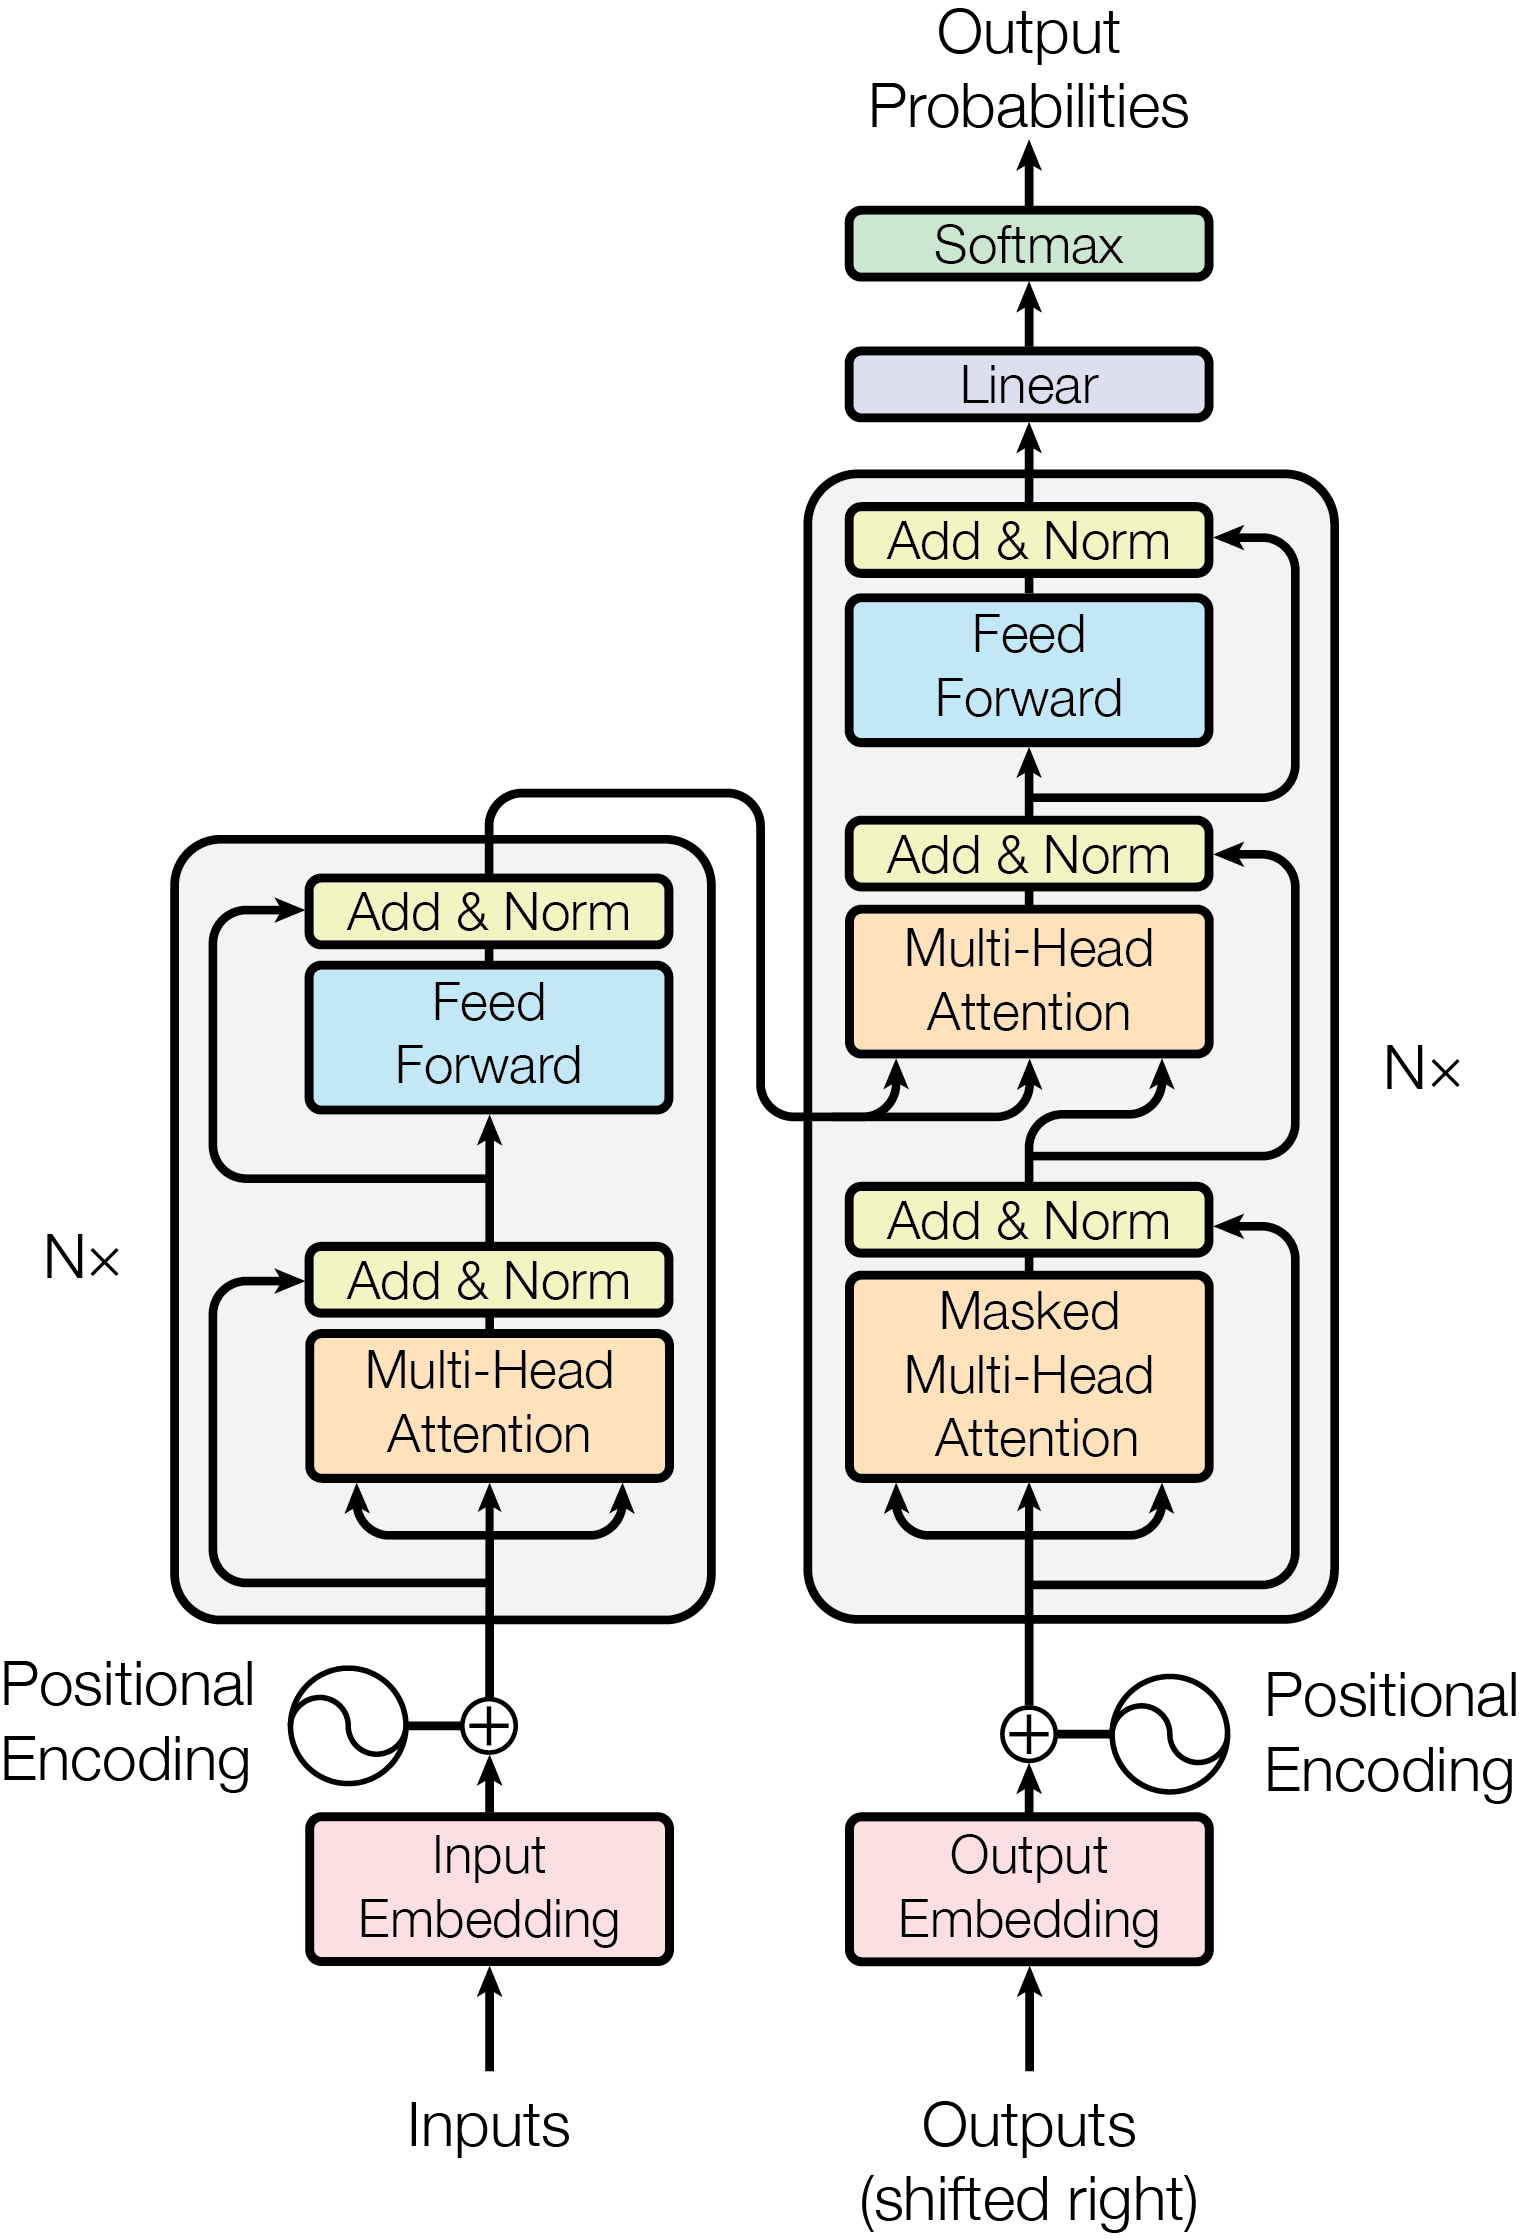
\includegraphics[width=0.5\linewidth]{figs/lec2/lec2.01.png}
  \caption{The Transformer-model architecture}
  \label{fig: Transformer architecture}
\end{figure}

\clearpage
如图Figure \ref{fig: Transformer architecture}所示,Transformer由
\begin{enumerate}
  \item \textbf{Input Embedding}
  \item \textbf{Positional Encoding}
  \item \textbf{Encoder 结构}: Self-Attention, Feed-Forward
    % \begin{enumerate}
    %   \item \textbf{Multi-Head Self-Attention} + \textbf{Add \& Norm}
    %   \item \textbf{Feed-Forward} + \textbf{Add \& Norm}
    % \end{enumerate}
  \item \textbf{Decoder 结构}: Masked self-Attention, Encoder Attention, Feed-Forward
    % \begin{enumerate}
    %   \item \textbf{Masked Multi-Head Self-Attention} + \textbf{Add \& Norm}
    %   \item \textbf{Encoder–Decoder Attention} + \textbf{Add \& Norm}
    %   \item \textbf{Feed-Forward} + \textbf{Add \& Norm}
    % \end{enumerate}
  \item \textbf{Output Projection \& Softmax}
\end{enumerate}
这几个模块组成,整体是Encoder-Decoder结构,其中Encoder和Decoder均由多个相同的层堆叠而成,我们称其为Transformer Block。接下来,我们会逐个介绍这些模块。

\clearpage

{\chaptoc\noindent
\begin{minipage}[inner sep=0,outer sep=0]{0.9\linewidth}
  \subsection{Input Embedding}
\end{minipage}}

\Insight{Input Embedding}{将输入的文本序列通过tokenizer转化为token再由embedding method转化为模型可以处理的数值向量。}

\begin{figure}[htbp]
  \centering
  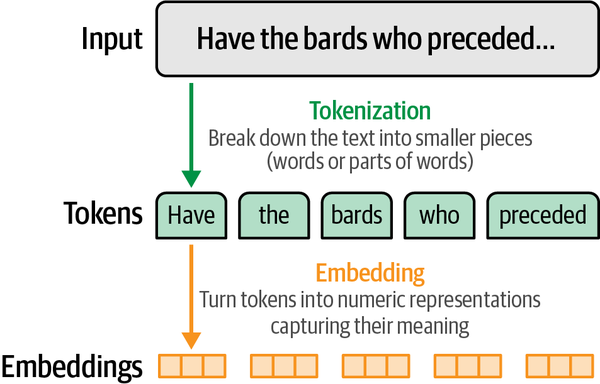
\includegraphics[width=0.5\linewidth]{figs/lec2/lec2.02.png}
  \caption{Input $\xrightarrow{}$ Tokens $\xrightarrow{}$ Embedding Vectors}
  \label{fig:Input Embedding Box}
\end{figure}

\subsubsection{Tokenization} 
请参考Lecture1 Section 4
\subsubsection{Embedding}

\textbf{{\color{tred} Goal: Find the best numerical representation for these tokens that the model can use to calculate and properly model the patterns in the text.}}

\Definition{Embedding Conversion}{Transforming these tokens into numerical representations that capture their meaning and patterns.}

\paragraph{1. Static Token Embeddings vs. Contextualized Embeddings}
\begin{itemize}
    \item \textbf{Static Token Embeddings}:为每个 token 分配一个唯一且固定的向量表示,常见实现包括 word2vec、GloVe 及 fastText 等。它们在大规模语料上预先训练完成后,每个 token 的向量在任意上下文中均保持不变。
    \begin{itemize}
        \item 优点:查表快速、计算开销小
        \item 缺点:无法区分同形异义词
    \end{itemize}
    \item \textbf{Contextualized Embeddings}:由基于语言模型在前向传播时动态生成。模型会结合整个输入序列及其邻近信息,对同一 token 产生不同的向量,实现语义消歧与更丰富的表达。
\end{itemize}

\begin{figure}[H]
  \centering
  \begin{subfigure}[t]{0.45\linewidth}
    \centering
    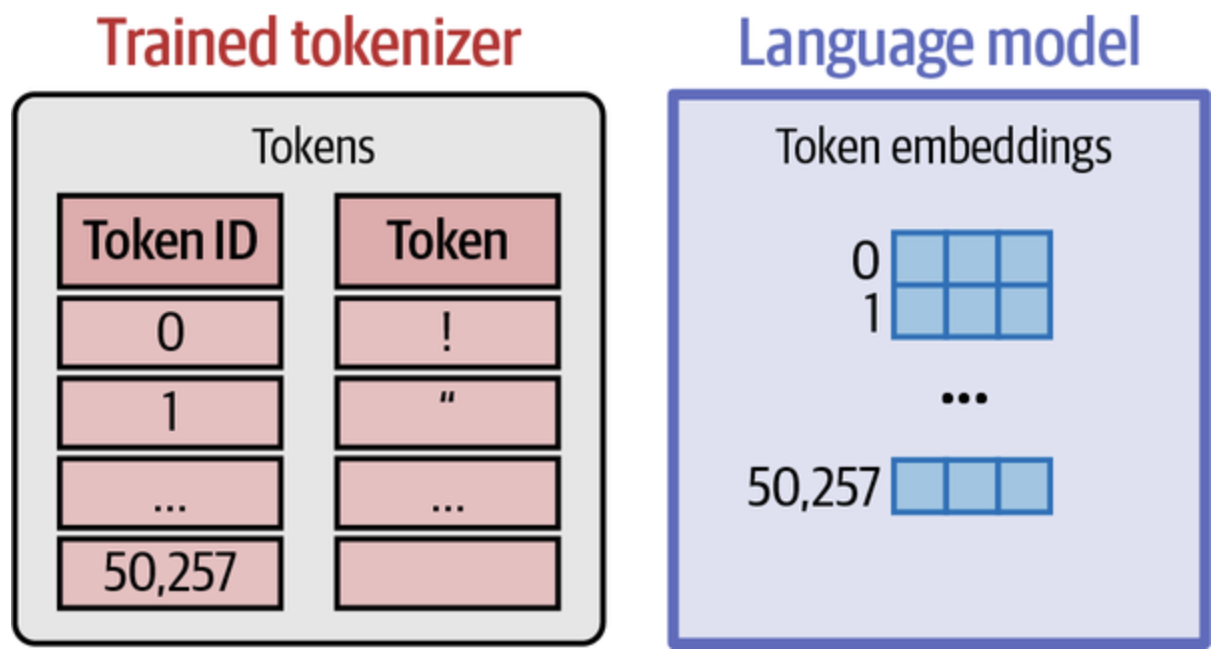
\includegraphics[width=\linewidth]{figs/lec2/lec2.03.png}
    \caption{Static Embedding}
    \label{fig:static-embedding}
  \end{subfigure}
  \hfill
  \begin{subfigure}[t]{0.45\linewidth}
    \centering
    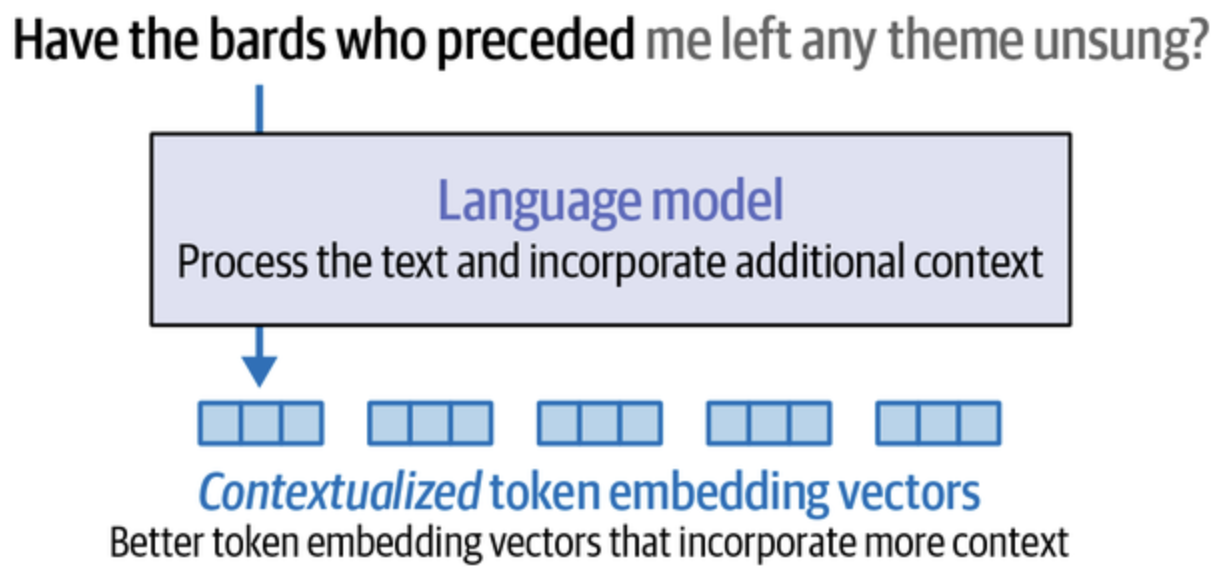
\includegraphics[width=\linewidth]{figs/lec2/lec2.04.png}
    \caption{Contextualized Embedding}
    \label{fig:contextualized-embedding}
  \end{subfigure}
  \caption{静态嵌入 vs. 上下文化嵌入对比}
  \label{fig:embeddings-comparison}
\end{figure}

\MarginImageWithNote
  {figs/lec2/lec2.05.png}
  {\captionof{figure}{A language model operates on raw, static embeddings as its input and produces contextual text embeddings.}}

\paragraph{2. Text and Sentence Embeddings}~{}
        
\Definition{Text/Sentence Embeddings}{Use a single vector to represent the text/ sentence instead of just one token and captures its meaning.}




为了对整个句子、段落或文档进行语义表示,通常需要将多个 token 嵌入合成为一个定长向量。常见方法包括:
\begin{itemize}
  \item \textbf{Mean Pooling(平均池化)}:对模型输出的所有 token 嵌入取序列维平均,
  \item \textbf{[CLS] 向量}:对于 BERT 系列模型,直接使用序列开头的 \texttt{[CLS]} 对应隐藏状态 \(\mathbf{h}_\text{[CLS]}\) 作为整句表示,无需额外聚合操作。
  \item \textbf{专用 Sentence Embedding 模型}:如 Sentence-BERT、MPNet 等,在大规模语料上针对句子级任务微调,直接输出高质量的句子向量。
\end{itemize}

\paragraph{3. Word2Vec}~{}

在\href{https://arxiv.org/abs/1301.3781}{Efficient estimation of word representations in vector space} 提出了两种框架,分别是Continuous Bag-of-Words Model(CBOW)和Continuous Skip-gram Model. 


\begin{figure}[htbp]
  \centering
  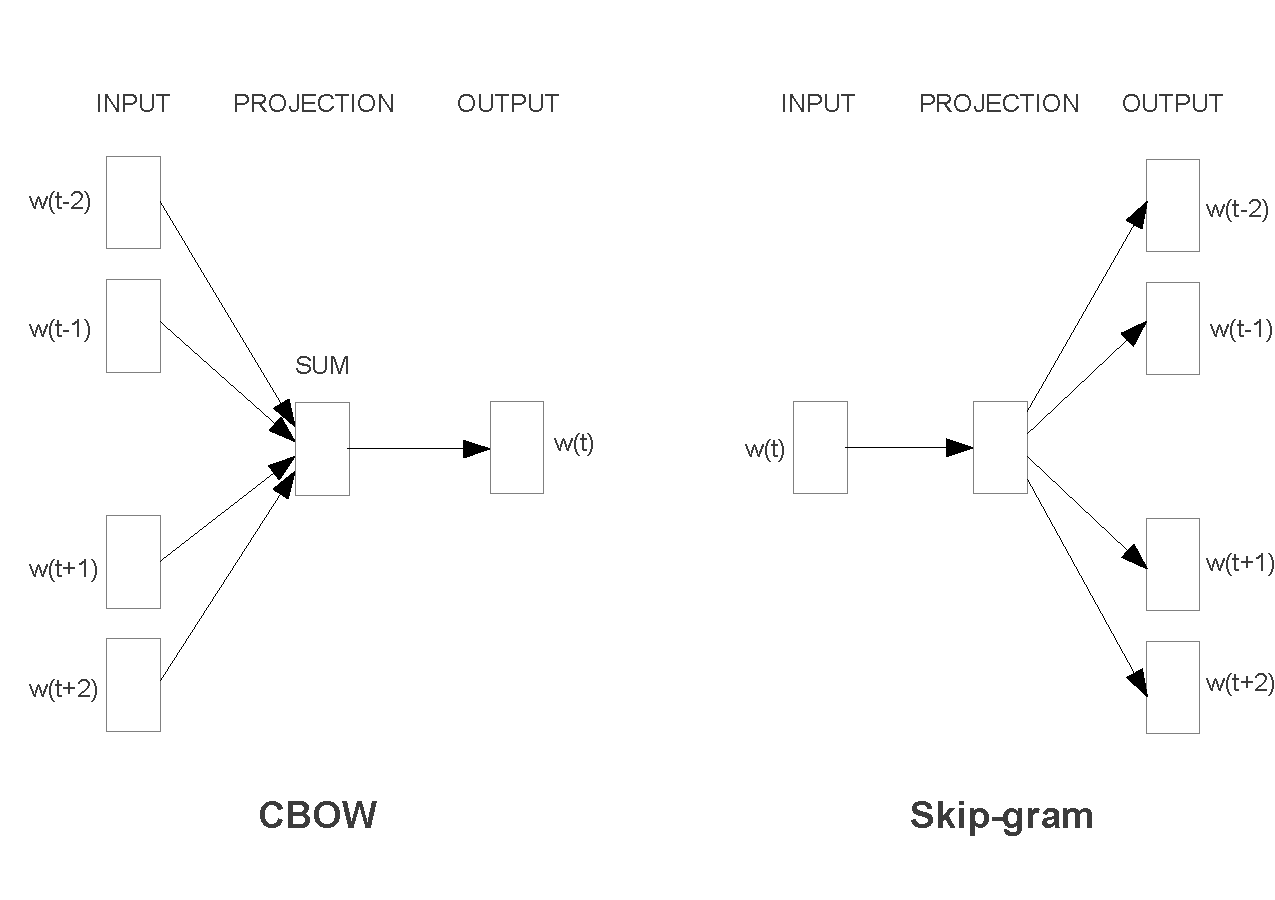
\includegraphics[width=0.5\linewidth]{figs/lec2/lec2.06.pdf}
  \caption{CBOW和Skip-gram architecture示意图}
  \label{fig:Word2Vec}
\end{figure}

\begin{itemize}
  \item \textbf{预测方向不同}:  
    CBOW 以上下文词(前后各 $m$ 个词)为输入,预测中心词 $w_t$;  
    Skip-gram 则以中心词 $w_t$ 为输入,分别预测其上下文词 $w_{t\pm j}$。  
  \item \textbf{输入输出结构}:  
    CBOW 将上下文词向量取平均或求和后输入,输出中心词的概率分布;  
    Skip-gram 对每个上下文位置都独立训练一个分类器,输出多个上下文词的分布。   
\end{itemize}



\clearpage
\subsection{Positional Encoding}
Transformer 的一个突破是完全基于注意力机制,去除了循环(RNN)和卷积(CNN)操作,这使得模型能够并行处理输入序列。然而,这也带来了一个问题:模型无法感知输入序列中各个 token 的相对或绝对位置。

为了让模型在注意力计算时感知每个 token 的位置信息,我们在输入的 embedding 中加入一个位置向量(Positional Encoding),使得每个 token 的表示不仅包含其语义信息,还包含其在序列中的位置信息。

具体来说,对于序列中位置 $pos$ 的 token,其最终输入表示为:
\[
\mathbf{z}_{pos} = \mathbf{e}_{pos} + \mathbf{p}_{pos}
\]
其中:
$\mathbf{e}_{pos} \in \mathbb{R}^{d_{\text{model}}}$ 为该 token 的词向量(token embedding);
$\mathbf{p}_{pos} \in \mathbb{R}^{d_{\text{model}}}$ 为对应位置的位置编码向量。

\paragraph{1.固定正余弦位置编码(Vaswani原版)}~{}
\\
\MarginImageWithNote
  {figs/lec2/lec2.07.png}
  {\captionof{figure}{位置编码示意图}}

在原始 Transformer 中,位置编码 $\mathbf{p}_{pos}$ 采用\textbf{固定的正余弦函数}形式:
\[
\text{PE}(pos, 2i) = \sin\left( \frac{pos}{10000^{2i / d_{\text{model}}}} \right), \quad
\text{PE}(pos, 2i+1) = \cos\left( \frac{pos}{10000^{2i / d_{\text{model}}}} \right)
\]
其中 $i$ 为向量维度的下标(从 0 开始),偶数维使用正弦,奇数维使用余弦。

这种编码方式的优势在于:
\begin{enumerate}
  \item \textbf{无参数}:不依赖训练,初始化即具备区分顺序的能力;
  \item \textbf{可外推}:支持推理时处理比训练时更长的序列;
  \item \textbf{保留相对位置信息}:任意两个位置的编码差值与它们的距离成规律性变化。
\end{enumerate}

\paragraph{2.可学习位置编码}~{}
\\
相比之下,另一种常用方法是可学习位置编码(Learnable Positional Embedding),即为每个位置直接分配一个可训练向量:
\[
\mathbf{p}_{pos} = \text{Embedding}(pos)
\]
这种方法的优点是灵活性强、可与任务数据更好适配,但在序列长度超过训练范围时,泛化能力可能较弱。

\begin{table}[H]
\centering
\begin{tabular}{|c|c|c|}
\hline
方法 & 优点 & 缺点 \\
\hline
正余弦位置编码 & 外推性好,无需训练 & 表达能力固定,灵活性低 \\
可学习位置编码 & 灵活性强,适应任务 & 外推性差,需额外参数 \\
\hline
\end{tabular}
\caption{两种常见位置编码方法的比较}
\end{table}


\clearpage
\subsection{Encoder 结构}
Encoder 有N个相同的层(Transformer Block)堆叠而成,每一层都包含两个子层:Multi-Head Self-Attention 和 Feed-Forward Network。每个子层后面都有一个残差连接(Add \& Norm)。

\MarginImageWithNote
  {figs/lec2/lec2.08.png}
  {\captionof{figure}{Transdormer Encoder Block from Vaswani et al. (2017)}}

每一个Transformer Block由两部分组成:
\begin{enumerate}
  \item \textbf{Attention层}:计算输入序列中各个 token 之间的关系,捕捉全局上下文信息。
  \item \textbf{Feed-Forward层}:对每个 token 的表示进行非线性变换,增强模型表达能力。  
\end{enumerate} 

\begin{figure}[htbp]
  \centering
  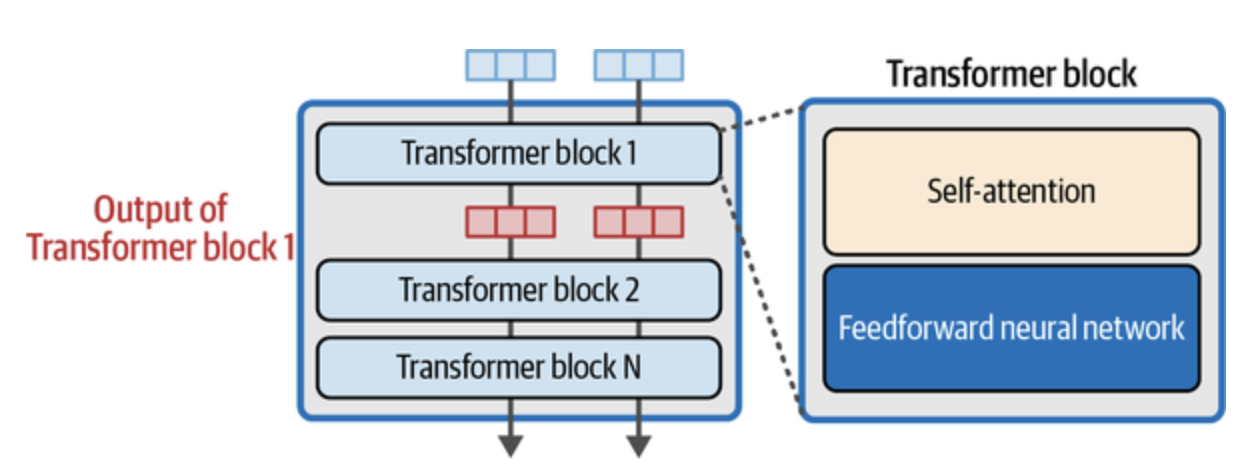
\includegraphics[width=1\linewidth]{figs/lec2/lec2.09.png}
  \captionof{figure}{Transformer Encoder Block from Vaswani et al. (2017)}
  \label{fig:Transformer Encoder Block}
\end{figure}

\subsubsection{多头自注意机制}
Attention机制主要做了两件事:
\begin{enumerate}
  \item A way to score how {\color{tred}relevant} each of the previous input tokens are to the current token being processed.

  \item Using those scores, we {\color{tred}combine the information} from the various positions into a single output vector.
\end{enumerate}   


To give the Transformer more extensive attention capability, the attention mechanism is {\color{tred}duplicated and executed multiple times in parallel}. Each of these parallel applications of attention is conducted into an {\color{dblue}\textit{attention head}}. This increases the model’s capacity to model complex patterns in the input sequence that require paying attention to different patterns at once.

\begin{figure}[htbp]
  \centering
  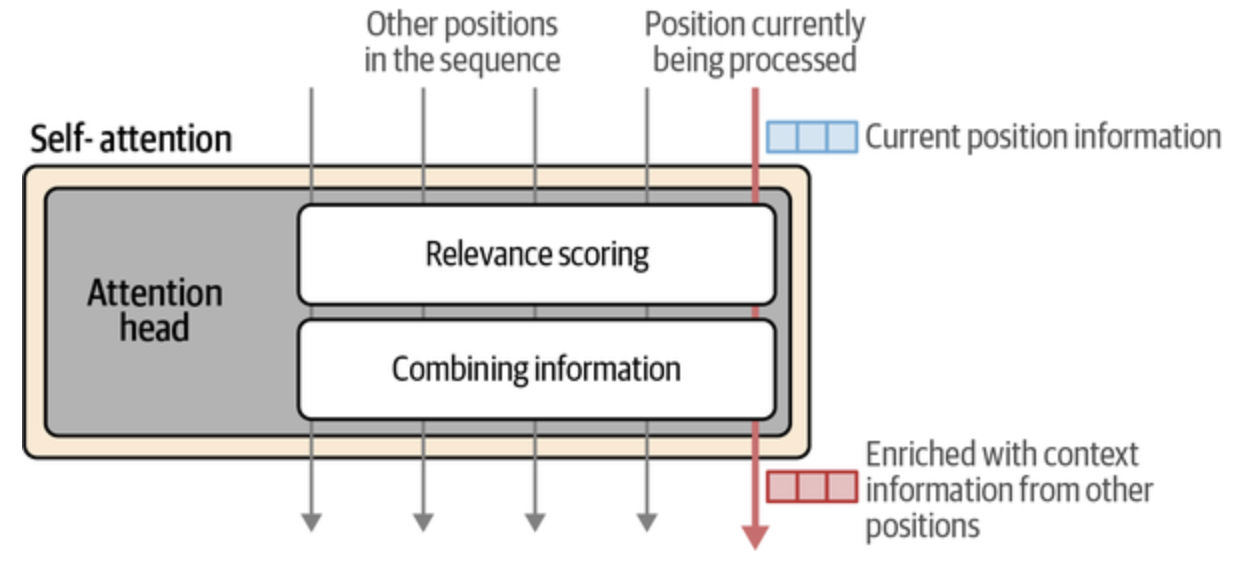
\includegraphics[width=0.6\linewidth]{figs/lec2/lec2.10.png}
  \caption{We get better LLMs by doing attention multiple times in parallel, increasing the model’s capacity to attend to different types of information.}
  \label{fig:Multi-Head Attention}
\end{figure}

\clearpage  
在原版的Transformer中,Multi-Head Self-Attention的计算图如下:
\begin{figure}[htbp]
  \centering
  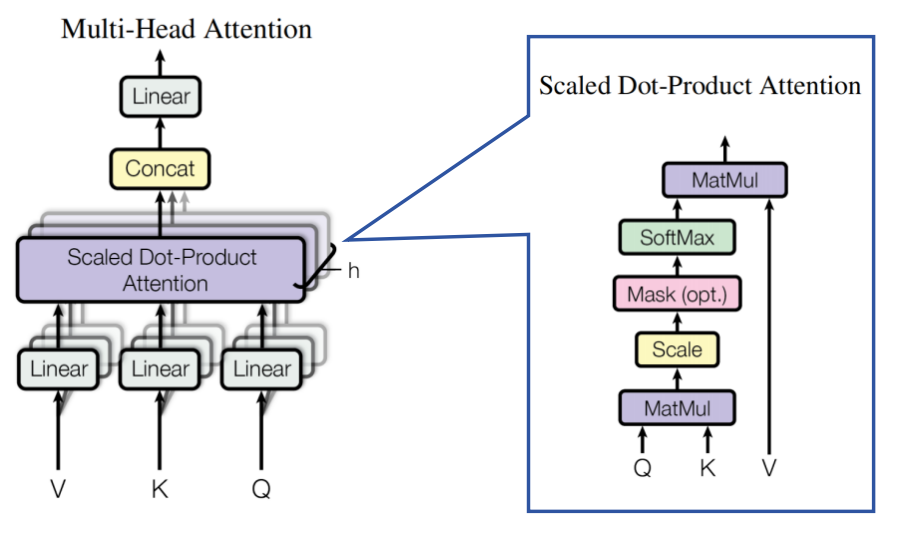
\includegraphics[width=0.75\linewidth]{figs/lec2/lec2.11.png}
  \caption{Multi-Head Self-Attention计算图}
  \label{fig:Multi-Head Self-Attention计算图}
\end{figure}

\MarginNote{

\Remark{
\textbf{Self-Attention 与 Attention 的区别}:
\begin{itemize}
  \item \textbf{Attention} 是一种通用机制,Query、Key、Value 可以来自不同的序列或不同模态的数据。例如在机器翻译中,编码器输出作为 Key/Value,解码器当前状态作为 Query,这被称为 \emph{cross-attention}。
  \item \textbf{Self-Attention} 是 Attention 的一种特殊情况,其中 Query、Key、Value 都来自同一组输入序列。它的作用是在同一序列内部建立位置之间的依赖关系,让每个位置能够根据相关性动态融合来自其他位置的信息。
\end{itemize}}  

}


Attention 其实就是一个加权求和的过程,可以看作是对输入向量的加权平均。其核心公式为:
\begin{equation}
\text{Attention}(Q, K, V) = \text{softmax} \left( \frac{Q K^\mathsf{T}}{\sqrt{d_k}} \right) V
\end{equation}  
其中:
\begin{itemize}
    \item $Q$(Query):表示当前 token 想要从其他位置“检索”信息的需求,决定当前 token 想找什么信息;
    \item $K$(Key):表示每个 token 的“特征标签”,决定每个 token 能被匹配成什么信息;
    \item $V$(Value):表示实际要被传递或聚合的内容,决定每个 token 能提供什么信息;
    \item $d_k$:缩放因子,用于防止点积结果过大导致梯度消失。
\end{itemize}

\QA{如何获得$Q$,$K$,$V$三个矩阵}
{
\\
\textbf{训练阶段}:
设当前层输入为 $X \in \mathbb{R}^{n \times d_{\text{model}}}$(已包含 token embedding 与位置编码),
每个注意力头 $i$ 具有三组可训练权重矩阵:
\[
W_Q^{(i)} \in \mathbb{R}^{d_{\text{model}} \times d_k},\quad
W_K^{(i)} \in \mathbb{R}^{d_{\text{model}} \times d_k},\quad
W_V^{(i)} \in \mathbb{R}^{d_{\text{model}} \times d_v}.
\]
(可选偏置 $b_Q^{(h)},b_K^{(h)},b_V^{(h)}$)。则有
通过线性投影计算:
\[
Q^{(i)} = X W_Q^{(i)} + b_Q^{(i)},\quad
K^{(i)} = X W_K^{(i)} + b_K^{(i)},\quad
V^{(i)} = X W_V^{(i)} + b_V^{(i)}.
\]
训练过程中,\textbf{反向传播(backpropagation)}会更新 $W_Q^{(i)},W_K^{(i)},W_V^{(i)}$,而 $Q,K,V$ 仅是中间结果,不直接被存储或训练。

\medskip
\textbf{预测阶段}:
使用训练好的 $W_Q^{(i)},W_K^{(i)},W_V^{(i)}$ 对当前输入 $X$ 重新计算 $Q,K,V$。
在自回归生成任务中,会缓存历史步骤的 $K,V$(KV~cache),
新生成 token 时仅需计算其对应的 $Q$(及自身 $K,V$),并与缓存的 $K,V$ 进行注意力计算,从而避免重复计算、加速推理。
}
我们将用一个Attention Head来说明Attention的计算过程,因为其余的heads除了投影矩阵($W_Q^{(i)}$,$W_K^{(i)}$,$W_V^{(i)}$)不同,其他计算过程是一样的。
\paragraph{Step0:进行Self-Attention之前的输入和投影矩阵}~{}
\begin{figure}[htbp]
  \centering
  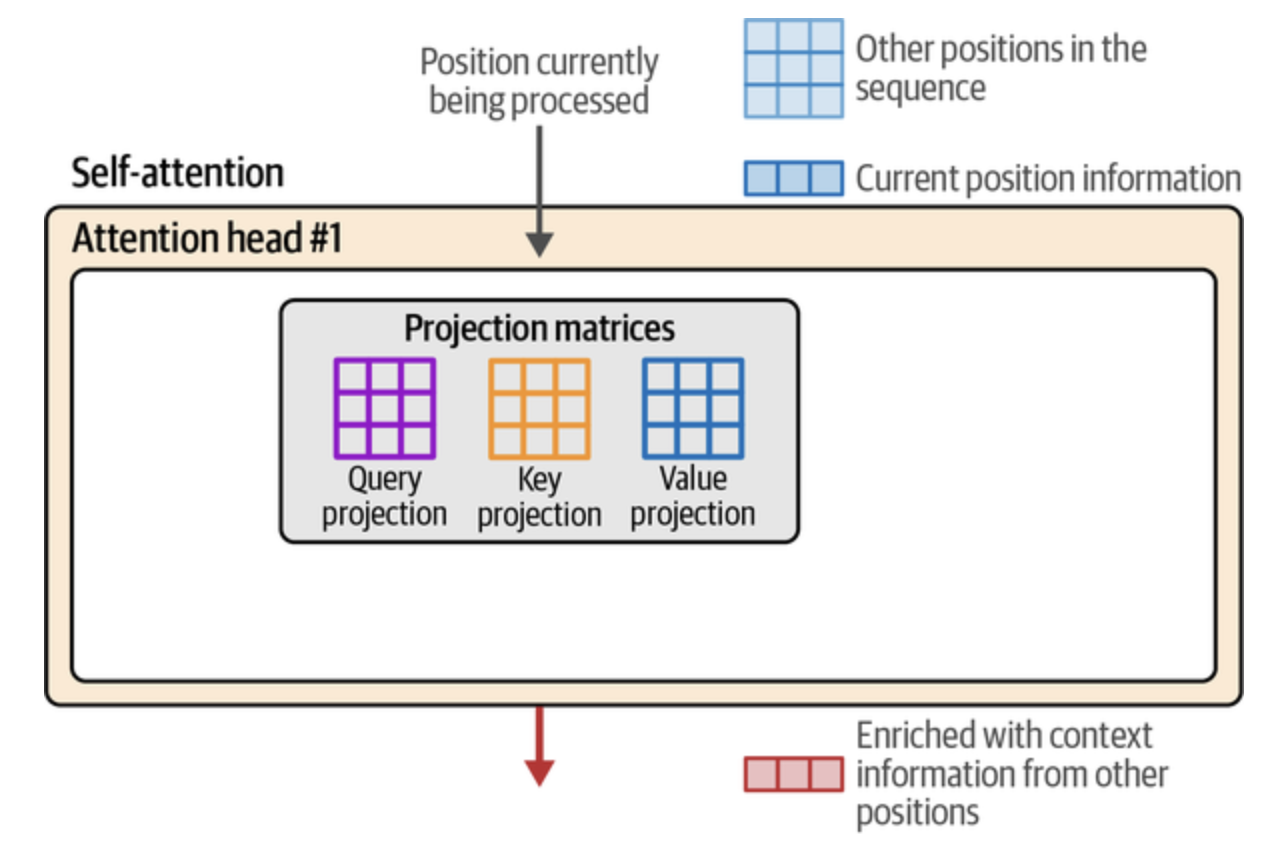
\includegraphics[width=0.8\linewidth]{figs/lec2/lec2.12.png}
  \caption{Step0:进行Self-Attention之前的输入和投影矩阵}
  \label{fig:Step0:进行Self-Attention之前的输入和投影矩阵}
\end{figure}

\noindent\textbf{输入:}
\begin{itemize}
  \item {\color{dblue}Current position information}:当前 token 的词向量(token embedding)与位置编码(positional encoding)之和。
  \item 之前所有 token 的向量表示(同样包含词向量和位置编码)。
\end{itemize}

\noindent\textbf{三个投影矩阵:}
\begin{itemize}
  \item {\color{qpurple}Query Projection} $W_Q$:将输入映射到查询空间,表示当前 token 想要从其他 token 获取的信息类型。
  \item {\color{orange}Key Projection} $W_K$:将输入映射到键空间,表示每个 token 能被匹配成什么信息。
  \item {\color{zblue}Value Projection} $W_V$:将输入映射到值空间,表示每个 token 能提供的具体信息。
\end{itemize}

\noindent\textbf{输出:}
\begin{itemize}
  \item {\color{tred}Enriched with context information from other positions}:融合了与当前 token 高度相关的其他 token 信息后的新表示,既包含自身信息,也包含上下文信息。
\end{itemize}

\clearpage
\paragraph{Step1:根据投影矩阵更新$Q$,$K$,$V$}~{}
\begin{figure}[htbp]
  \centering
  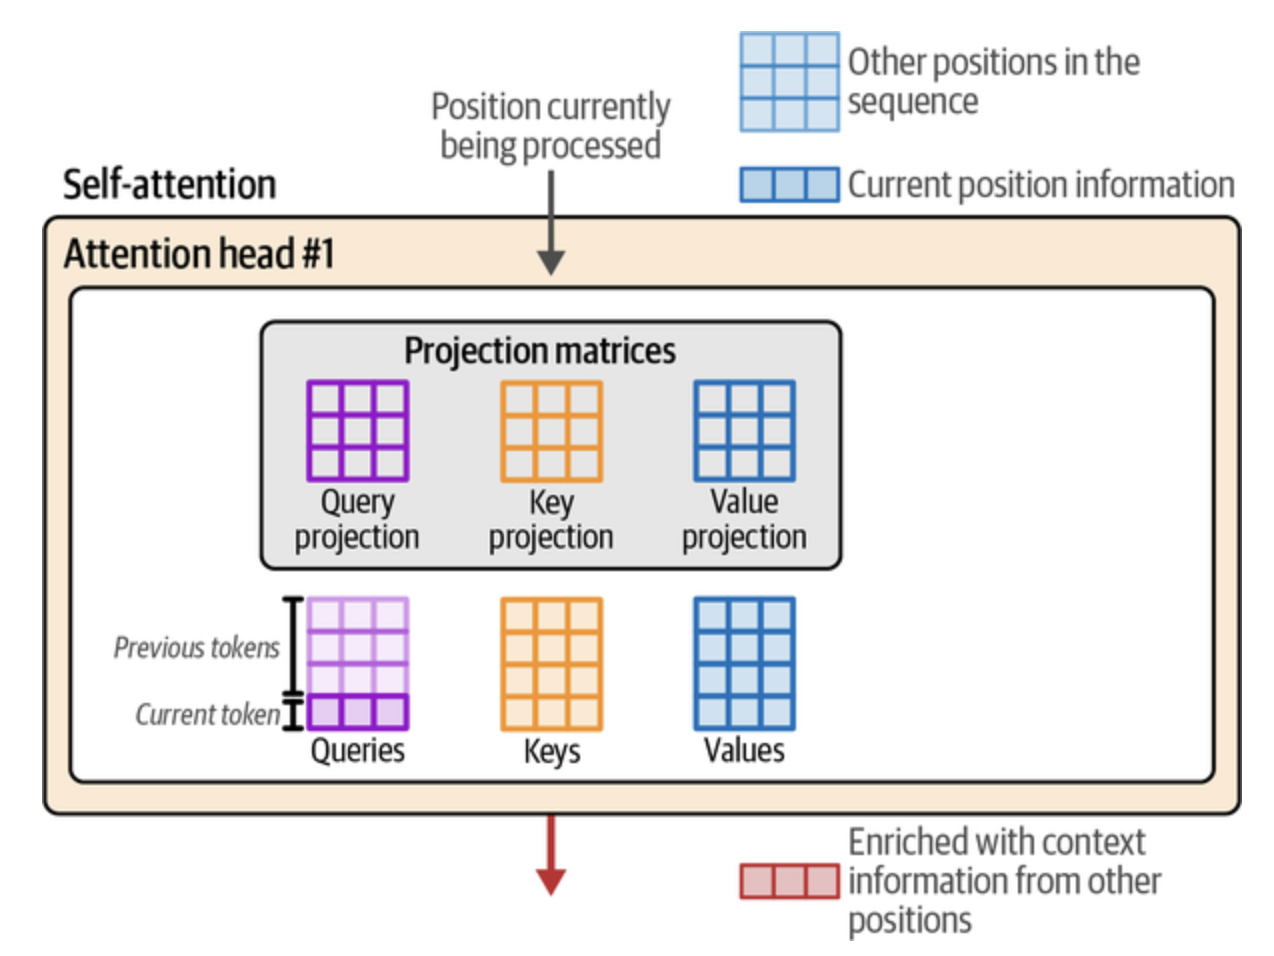
\includegraphics[width=0.8\linewidth]{figs/lec2/lec2.13.png}
  \caption{Step1:根据投影矩阵更新$Q$,$K$,$V$}
  \label{fig:Step1:根据投影矩阵更新$Q$,$K$,$V$}
\end{figure}

在该步骤中,输入矩阵 $X \in \mathbb{R}^{n \times d_{\text{model}}}$(由{\color{dblue}current position information和other positions in the sequence}组成) 会分别与三个可训练的投影矩阵相乘:
\[
Q = X W_Q,\quad K = X W_K,\quad V = X W_V
\]
其中 $W_Q \in \mathbb{R}^{d_{\text{model}} \times d_k}$、$W_K \in \mathbb{R}^{d_{\text{model}} \times d_k}$、$W_V \in \mathbb{R}^{d_{\text{model}} \times d_v}$是在训练过程中得到的投影矩阵。

在 $Q, K, V$ 矩阵中,每一行对应序列中一个 token 的表示,其中最后一行是当前位置 token(即{\color{dblue}current position information})的 $Q$、$K$、$V$ 向量。

这三个矩阵将在后续步骤中完成 Attention 的两个核心功能:
\begin{itemize}
  \item 计算相关性分数(Relevance scoring)
  \item 结合上下文信息(Combining information)
\end{itemize}

\clearpage
\paragraph{Step2:计算相关性分数并进行Softmax归一化}~{}
\begin{figure}[htbp]
  \centering
  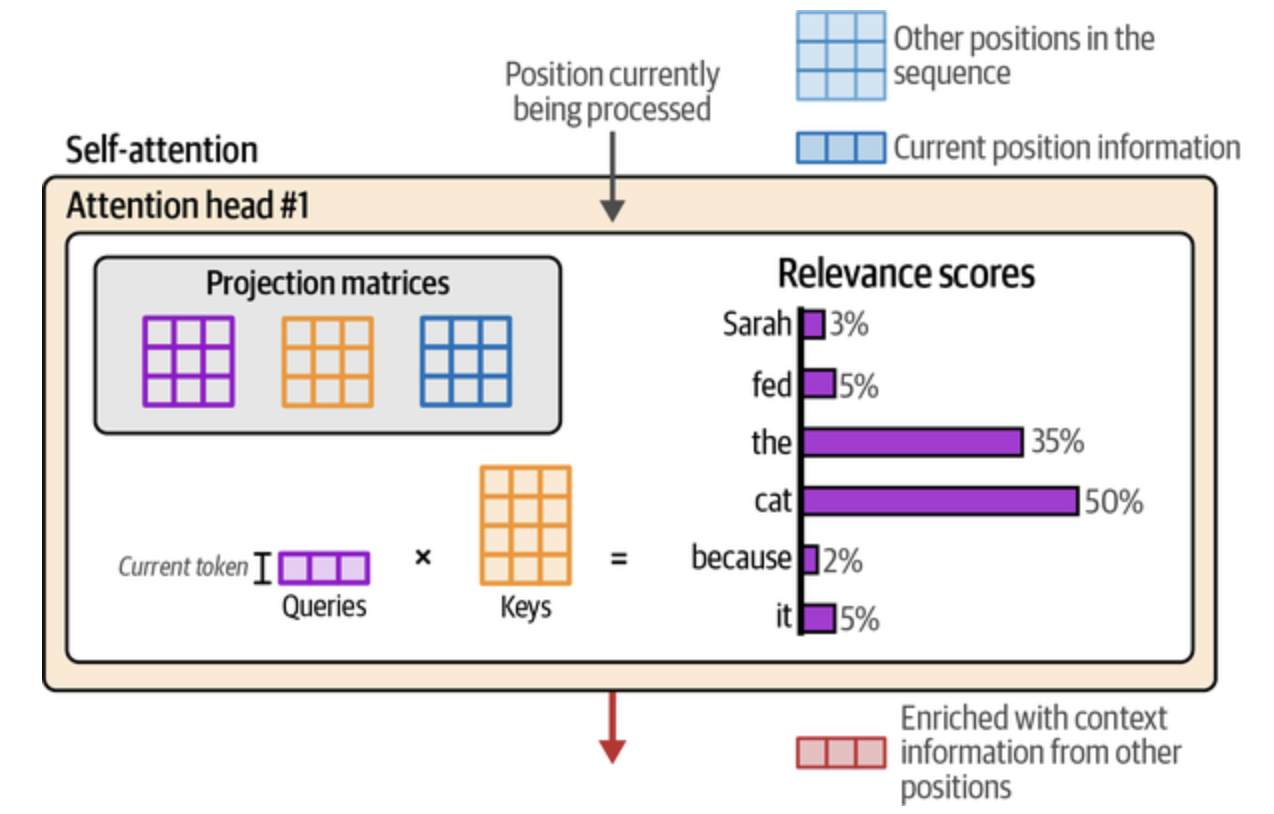
\includegraphics[width=0.8\linewidth]{figs/lec2/lec2.14.png}
  \caption{Step2:计算相关性分数并进行Softmax归一化}
  \label{fig:Step2:计算相关性分数并进行Softmax归一化}
\end{figure}

在 {\color{qpurple}相关性计算(Relevance scoring)} 步骤中,首先将当前位置的查询向量与整个键矩阵相乘:
\[
\text{scores} = Q_{\text{current}} K^\mathsf{T}
\]
得到的分数表示当前位置与每个上下文 token 之间的匹配程度。为了避免分数随维度 $d_k$ 增大而导致梯度消失问题,这些分数会除以缩放因子 $\sqrt{d_k}$ 进行归一化。  

随后,将缩放后的分数输入 Softmax 函数,得到一个概率分布(所有权重之和为 1),该分布反映了模型在当前位置应如何分配对各个上下文 token 的注意力。  

因此,这一步对应公式(2.1)中的:
\[
\text{softmax}\left(\frac{QK^\mathsf{T}}{\sqrt{d_k}}\right)
\]

\MarginImageWithNote
{figs/lec2/lec2.16.png}
{\captionof{figure}{Teacher Forcing 示意图}\label{fig:TeacherForcing}}
{
\Definition{Teacher Forcing}{
一种序列到序列模型(seq2seq)常用的{\color{tred}训练策略}。在训练时,将真实的目标序列(ground truth)按时间步作为解码器的输入,而不是使用模型上一步的预测结果。这样可以一次性并行计算整个序列的输出,提升训练速度并稳定梯度。即$Q$为完整矩阵。
}\label{def:teacher-forcing}

\Definition{Auto-regressive Model}{
一种{\color{tred}序列生成}方式,模型按时间顺序逐个生成 token。每一步的输出仅依赖于先前生成的 token(满足因果掩码约束,不能看到未来 token)。在推理时需要顺序计算,但可以利用缓存机制(KV cache)加速。即Q为仅包含当前位置的向量 $Q_{\text{current}}$。
}\label{def:auto-regressive}

}

\Insight{训练与推理中的计算方式的不同}{
\begin{itemize}
\item  \textbf{训练阶段:Teacher Forcing}  \\
$Q$、$K$、$V$ 都是完整的矩阵,模型可以同时计算序列中所有位置的相关性分数。

\item \textbf{推理阶段:Auto-regressive}\\
计算是逐位置进行的:$Q$ 退化为仅包含当前位置的一个向量 $Q_{\text{current}}$,它会与缓存的 $K$、$V$(KV Cache)交互计算注意力权重,从而逐步生成序列。批量推理可以同时处理多个序列,但同一序列内部的 token 必须按顺序生成。
\end{itemize}
}



\clearpage

\paragraph{Step3:用注意力权重对$𝑉$权求和,得到输出}~{}
\begin{figure}[htbp]
  \centering
  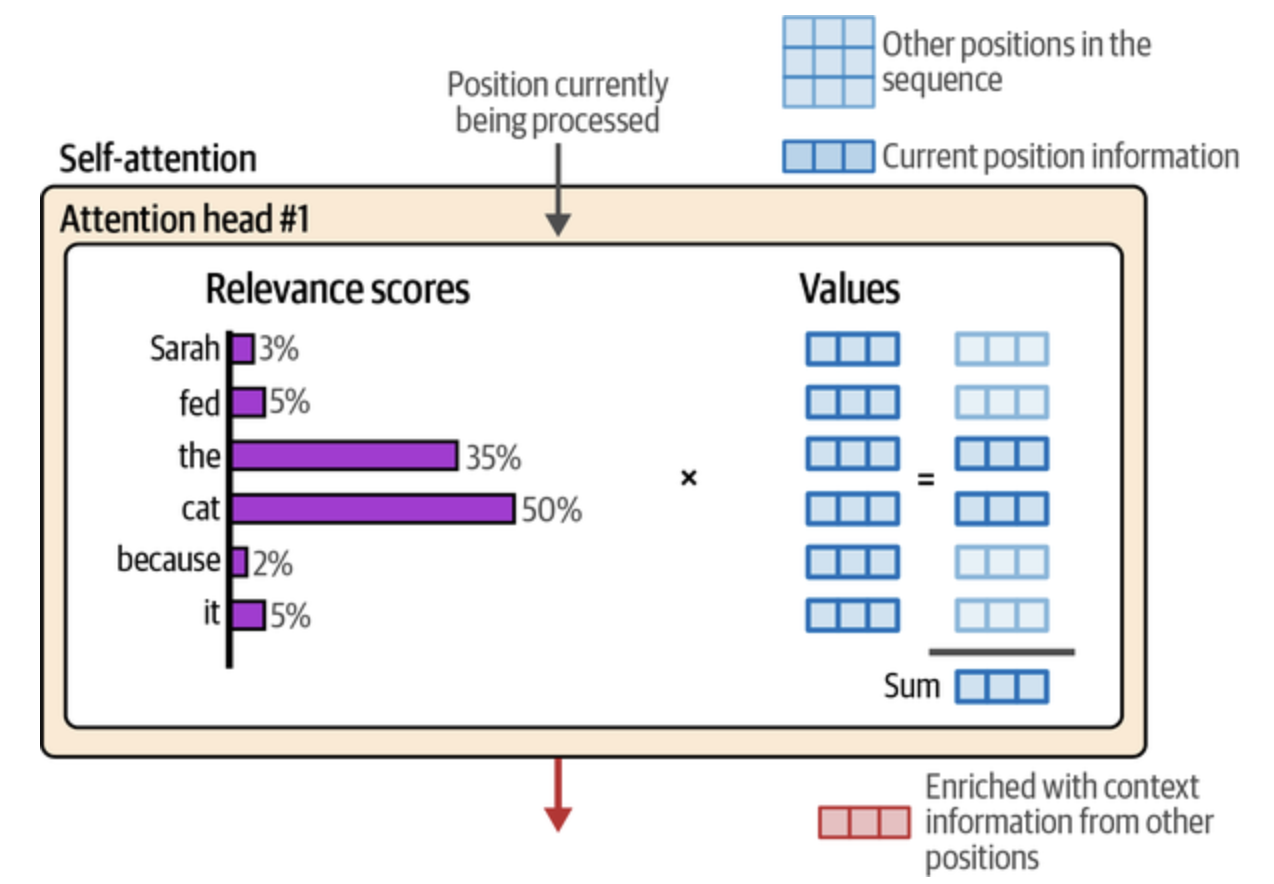
\includegraphics[width=0.8\linewidth]{figs/lec2/lec2.15.png}
  \caption{Step3:用注意力权重对$𝑉$权求和,得到输出}
\label{fig:Step3:用注意力权重对$𝑉$权求和,得到输出}
\end{figure}

在获得注意力权重  {\color{qpurple}relevance scores} 之后,当前位置会使用这些权重对值矩阵 $V$ 进行加权求和:  
\[
\text{Output}_{\text{current}} = \sum_{i=1}^{n} \alpha_i V_i
\]
其中 $\alpha_i$ 是当前位置对第 $i$ 个 token 的注意力权重(Softmax 输出的概率),$V_i$ 是该 token 在值矩阵中的向量表示。  

这一加权求和操作,使得当前位置的输出向量不仅保留了自身的语义信息,还融合了来自其他位置的重要上下文信息({\color{tred}Enriched with context information from other positions})。  

因此,这一步对应公式(2.1)中的:
\[
\text{Output} = \text{softmax}\left(\frac{QK^\mathsf{T}}{\sqrt{d_k}}\right) V
\]
其中,\(\text{softmax}\left(\frac{QK^\mathsf{T}}{\sqrt{d_k}}\right)\) 可记作注意力权重矩阵 \(\alpha\),表示当前位置对各个 token 的注意力分布。


\clearpage
\paragraph{Step4: 多头注意力的输出合并}~{}

在前面的步骤中,我们详细解释了一个 \emph{Attention Head} 的计算过程:通过将输入投影为 $Q$、$K$、$V$,计算相关性分数并进行加权求和,从而生成融合上下文信息的输出表示。  

然而,一个 Attention Head 在一次计算中只能在\textbf{同一个表示子空间}中学习位置间的依赖关系。为了让模型在不同的特征子空间中\emph{同时}捕捉多种模式(例如语义关系、句法结构、长程依赖等),Transformer 会将注意力机制\textbf{复制多份并行执行},形成多个独立的 Attention Head。

\begin{figure}[htbp]
  \centering
  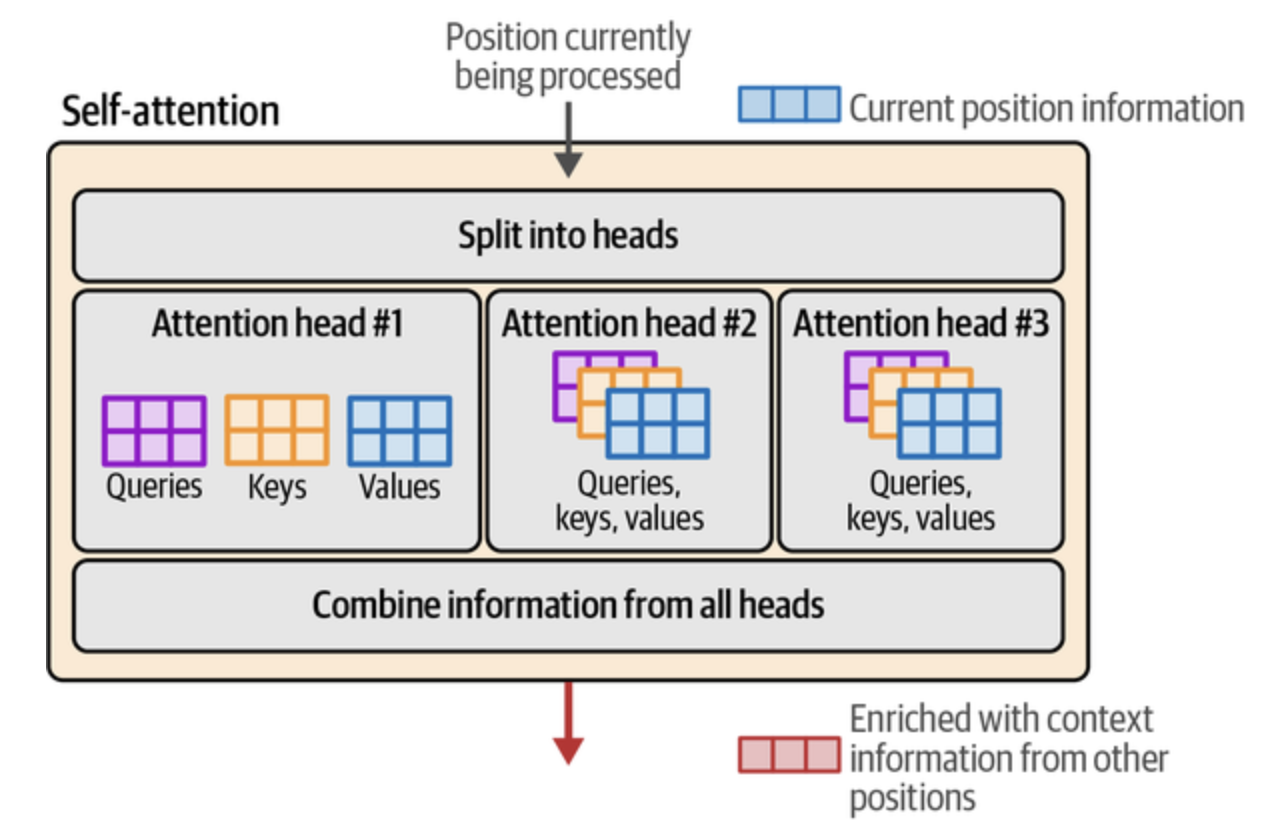
\includegraphics[width=0.8\linewidth]{figs/lec2/lec2.17.png}
  \caption{Multi-Head Attention中的$Q$,$K$,$V$在不同Head中是独立的}
  \label{fig:Multi-Head Attention计算图}
\end{figure}

\MarginImageWithNote
  {figs/lec2/lec2.18.png}
  {\captionof{figure}{Multi-Head Attention的输出拼接示意图}}


\MarginImageWithNote
  {figs/lec2/lec2.19.png}
  {\captionof{figure}{多头注意力输出整合并送入FFN}}
  {
\begin{enumerate}
  \item \textbf{拼接各个注意力头的输出}  
  将 $Z_0, Z_1, \dots, Z_{h-1}$ 在特征维度上进行拼接,得到拼接后的矩阵:
  \[
  Z_{\text{concat}} = \text{Concat}(Z_0, Z_1, \dots, Z_{h-1})
  \]
  
  \item \textbf{线性变换整合信息}  
  将 $Z_{\text{concat}}$ 乘以一个可训练的投影矩阵 $W^O$,得到最终的多头注意力输出:
  \[
  Z = Z_{\text{concat}} W^O
  \]
  这个过程的作用是将多个头的特征重新整合到模型的表示空间,使不同子空间的信息能够交互融合。

  \item \textbf{送入后续的前馈神经网络(FFN)}  
  最终的 $Z$ 会作为后续 Point-Wise FFN 的输入,进一步进行非线性变换和特征提取。
\end{enumerate}
}

在原始 Transformer 论文中,Multi-Head Self-Attention 的定义为:
\[
\text{MultiHead}(Q, K, V) = \text{Concat}(\text{head}_1, \dots, \text{head}_h) W^O
\]
其中:
\[
\text{head}_i = \text{Attention}(Q W_i^Q, K W_i^K, V W_i^V)
\]
\begin{itemize}
  \item $h$ 是头的数量;
  \item $W_i^Q, W_i^K, W_i^V$:第 $i$ 个 Head 的可训练投影矩阵; 
  \item $W^O$ 是最终的线性变换矩阵,将拼接后的向量映射回模型维度 $d_{\text{model}}$。
\end{itemize} 
 

在多头注意力(Multi-Head Attention)中,不同的注意力头(Attention Head)可以从不同的子空间中捕捉序列的特征。  
完成每个注意力头的计算后,得到多个输出矩阵:
\[
Z_0, Z_1, \dots, Z_{h-1}
\]
其中 $h$ 为注意力头的数量。




\clearpage
\paragraph{Step5: Add \& Norm}~{}

在 Transformer 中,每个子层(例如多头注意力层、前馈神经网络层)的输出都会经过 \textbf{残差连接(Residual Connection)} 与 \textbf{层归一化(Layer Normalization)},这一组合被称为 \textbf{Add \& Norm} 步骤。

\subparagraph{Layer Normalization}  
Layer Normalization(层归一化)对每个位置(token)的表示向量单独进行归一化,从而使模型在训练时更加稳定并加快收敛。  
其核心思想是:对每个位置的向量 $\mathbf{x}$ 进行均值与方差的归一化处理:
\[
\text{LayerNorm}(\mathbf{x}) = \frac{\mathbf{x} - \mu}{\sigma + \epsilon} \cdot \gamma + \beta
\]
其中:
\[
\mu = \frac{1}{d} \sum_{i=1}^{d} x_i, \quad
\sigma = \sqrt{\frac{1}{d} \sum_{i=1}^{d} (x_i - \mu)^2}
\]
\begin{itemize}
  \item $\mathbf{x} \in \mathbb{R}^d$:表示一个 token 的向量表示(embedding)。
  \item $\mu$、$\sigma$ 分别为该向量的均值和标准差。
  \item $d$ 为向量的维度(即 embedding size)。
  \item $\gamma, \beta$ 为可学习的缩放与平移参数。
  \item $\epsilon$ 是防止除零的小常数,通常取 $10^{-6}$。
\end{itemize}

与 Batch Normalization 不同,Layer Normalization 是\textbf{在特征维度上}进行归一化,而不是在 batch 维度上,因此更适合处理不同长度的序列。LN 对每个位置(token)单独归一化,避免了 BN 在可变序列、小 batch 以及自回归生成中可能出现的信息泄漏和统计不稳定问题。

\begin{figure}[htbp]
  \centering
  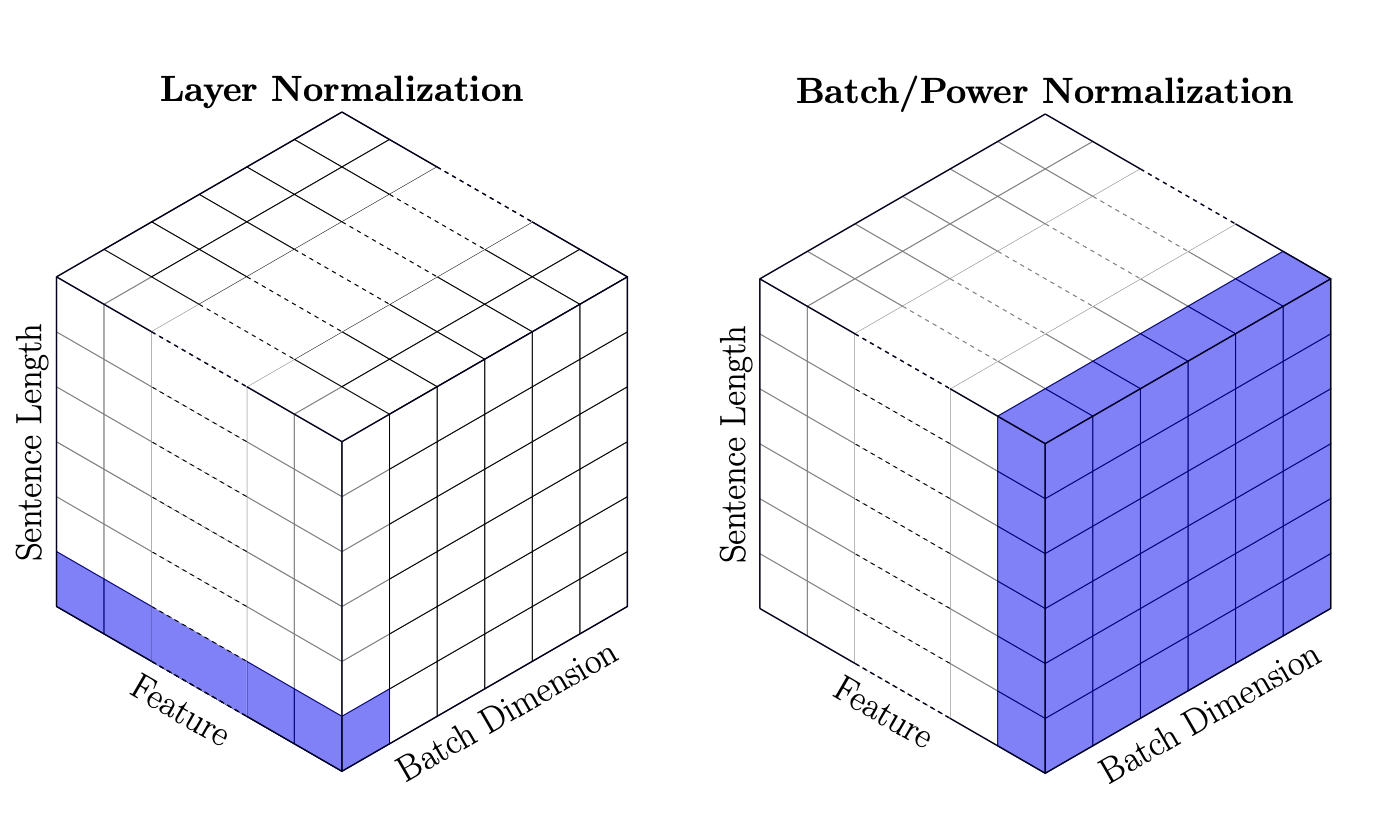
\includegraphics[width=0.6\linewidth]{figs/lec2/lec2.20.png}
  \caption{\href{http://proceedings.mlr.press/v119/shen20e/shen20e.pdf}{Layer Normalization vs. Batch Normalization} 示意图}
  \label{fig:layernorm}
\end{figure}

\clearpage
\subparagraph{Residual Connection}  
Residual Connection 通过将子层的输出与其输入相加:
\[
\mathbf{y} = \mathrm{Sublayer}(\mathbf{x}) + \mathbf{x}
\]

\MarginImageWithNote
  {figs/lec2/lec2.21.png}
  {\captionof{figure}{Residual Connection 示意图}}

为模型提供了一条直接的“恒等映射”路径(Identity Mapping),使得网络更容易学习到接近恒等变换的功能,从而缓解深层网络的退化问题。

在反向传播中,残差连接为梯度提供了两条路径:  
\begin{align}
\frac{\partial \mathcal{L}}{\partial \mathbf{x}}
&= \frac{\partial \mathcal{L}}{\partial \mathbf{y}} \cdot \frac{\partial \mathbf{y}}{\partial \mathbf{x}} \notag\\
&= \frac{\partial \mathcal{L}}{\partial \mathbf{y}} \cdot \left( \mathbf{I} + \frac{\partial \mathrm{Sublayer}(\mathbf{x})}{\partial \mathbf{x}} \right) \notag\\
&= \overset{\text{straight path}}{\frac{\partial \mathcal{L}}{\partial \mathbf{y}}}
\;+\;
\overset{\text{from output}}{\frac{\partial \mathcal{L}}{\partial \mathbf{y}}}
\,\cdot\,
\overset{\text{through the sub-layer}}{\frac{\partial\,\mathrm{Sublayer}(\mathbf{x})}{\partial \mathbf{x}}}
\tag{2.2}
\end{align}

第一项是直接传递的梯度,不依赖子层的计算结果,即使子层梯度趋近于 0,信息也不会完全丢失,从而有效缓解梯度消失问题。

\MarginNote{
\Definition{Constant Error Carousel (CEC)}{
CEC 是 LSTM(Long Short-Term Memory)结构中最核心的机制之一,用于在时间步之间“无衰减”地传递梯度,从而缓解 RNN 在长序列学习中容易出现的梯度消失问题。

在 LSTM 中,CEC 由单元状态(cell state)$c_t$ 及其恒等传递路径构成。当遗忘门 $f_t=1$ 且输入门 $i_t=0$ 时,$c_t$ 可以在多个时间步中保持不变,梯度在反向传播时也能沿这条路径稳定传递(即梯度近似为常数),因此称为 \textit{Constant Error Carousel}。

这一设计使得 LSTM 能够长期记忆关键信息,并在需要时通过门控机制有选择地更新或输出,从而有效建模长期依赖。
}
}
\Insight{Residual Connection 与 Constant Error Carousel(CEC)的联系}{
Residual Connection(残差连接)与 LSTM 中的 Constant Error Carousel(CEC)在梯度传播机制上有相似之处:

\begin{itemize}
  \item \textbf{共同点}:
    \begin{itemize}
      \item 都旨在缓解深层或长序列训练中的\textbf{梯度消失}问题。
      \item 都为梯度提供了\textbf{直通路径},使得反向传播时梯度可以不经过复杂的非线性变换直接传递。
      \item 都能在一定程度上保持信息在网络中的长期流动。
    \end{itemize}
  \item \textbf{区别}:
    \begin{itemize}
      \item Residual Connection 没有门控,输入与子层输出\textbf{恒等相加},结构更简单。
      \item CEC 在 LSTM 中配合门控机制(遗忘门 $f_t$、输入门 $i_t$)动态调节信息保留与更新的比例。
      \item Residual Connection 多用于深层前馈网络(如 Transformer),而 CEC 专注于循环结构中的长期依赖。
    \end{itemize}
\end{itemize}

可以将 Residual Connection 看作是 CEC 的\textbf{无门控恒等映射版本},虽缺乏动态调节能力,但在深层网络中已足够缓解梯度衰减。}



\clearpage
\subsubsection{Point-wise Feed-Forward Network}

\begin{figure}[htbp]
  \centering
  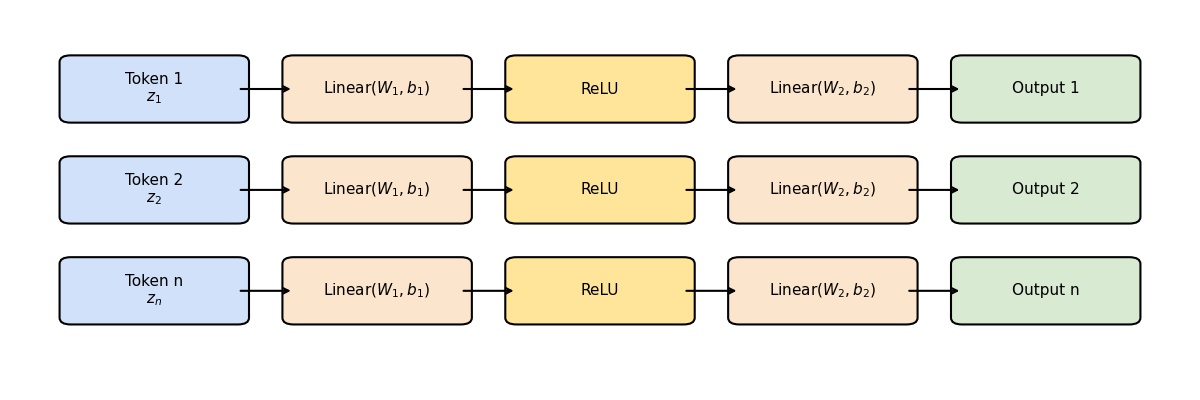
\includegraphics[width=0.6\linewidth]{figs/lec2/lec2.22.png}
  \caption{Point-wise Feed-Forward Network}
  \label{fig:Point-wise Feed-Forward Network}
\end{figure}

\textbf{输入:} 来自 Multi-Head Self-Attention 的输出矩阵
\[
Z \in \mathbb{R}^{n \times d_{\text{model}}}
\]
其中 $n$ 为序列长度,$d_{\text{model}}$ 为每个 token 的向量维度。
矩阵的每一行 $z_i$ 表示位置 $i$ 上的 token 表示,已经融合了来自其他位置的上下文信息。

\textbf{操作:} 对每一个位置的向量 $z_i$ 独立地应用相同的两层前馈网络和非线性激活:
\[
\text{FFN}(z_i) = \text{ReLU}(z_i W_1 + b_1) W_2 + b_2
\]
其中 $W_1, b_1, W_2, b_2$ 是在所有位置间共享的可学习参数。

\textbf{输出:} 
\[
Z' \in \mathbb{R}^{n \times d_{\text{model}}}
\]
矩阵的每一行 $z'_i = \text{FFN}(z_i)$,表示经过非线性变换后的 token 表示。

\textbf{目的:}
\begin{itemize}
    \item 在不改变位置间依赖关系的情况下,对每个位置的表示进行非线性特征变换。
    \item 与 Self-Attention 模块配合:Self-Attention 负责位置间的信息交互,FFN 负责位置内部的特征提炼。
    \item Point-Wise(逐位置)设计便于并行计算,且所有位置共享同一组参数,不随序列长度增加而膨胀。
\end{itemize}


\clearpage
\subsection{Decoder 结构}

Decoder 相较于Encoder有三个不同点:
\begin{itemize}
  \item \textbf{Masked Multi-Head Self-Attention}:在目标序列的自注意力中加入\textbf{因果 Mask(Causal Mask)},确保在训练过程中当前位置只能关注到自己和之前的 token,避免在训练时“偷看”未来信息。
  \item \textbf{Encoder-Decoder Attention(Cross-Attention)}:利用 Encoder 的输出作为 Key/Value,当前 Decoder 的隐藏状态作为 Query,实现对源序列信息的选择性关注。
  \item \textbf{Position-wise Feed Forward Network \& Add \& Norm}:与 Encoder 相同的前馈网络和残差归一化结构。
\end{itemize}


\subsubsection{Masked Multi-Head Self-Attention}


\MarginImageWithNote
  {figs/lec2/lec2.24.jpeg}
  {\captionof{figure}{Mask Matrix $M$示意图}\label{fig:Masked Multi-Head Self-Attention}}
  {
  其中:$M_{\text{causal}} \in \mathbb{R}^{n \times n}$ 是因果掩码矩阵,定义为:
  \[
  (M_{\text{causal}})_{ij} =
  \begin{cases}
  0 & j \le i \\
  -\infty & j > i
  \end{cases}
  \]
  当 $j > i$(未来位置)时,掩码值为 $-\infty$,Softmax 后对应权重为 0。
  }

Transformer 的 Decoder 采用 Masked Multi-Head Self-Attention 的原因是,在训练阶段我们通常使用 {\color{tred}\hyperref[def:teacher-forcing]{Teacher Forcing}}。  
这种方式虽然高效,但会导致 Decoder 在计算自注意力时可以“看到”当前位置之后的 token,即未来信息,从而造成数据泄露。  
为了避免这种“偷看”未来 token 的情况,我们需要在 Self-Attention 的相关性计算中引入掩码(mask)矩阵,将当前位置之后的注意力权重屏蔽为 0。  
在推理阶段{\color{dblue}\hyperref[def:auto-regressive]{Auto-regressive}}中,这种掩码同样适用,因为生成是逐步进行的。

具体来说,因果注意力(Causal Attention)的计算公式为:
\begin{equation}
\text{CausalAttention}(Q, K, V) = \text{softmax}\left(\frac{QK^\mathsf{T}}{\sqrt{d_k}} + M_{\text{causal}}\right)V
\tag{2.3}
\end{equation}


这种掩码机制保证了无论是在 Teacher Forcing 的训练阶段,还是在 Auto-regressive 推理阶段,当前位置的输出都只能依赖于当前位置及其之前的 token,从而严格遵守因果性约束。


\begin{figure}[htbp]
  \centering
  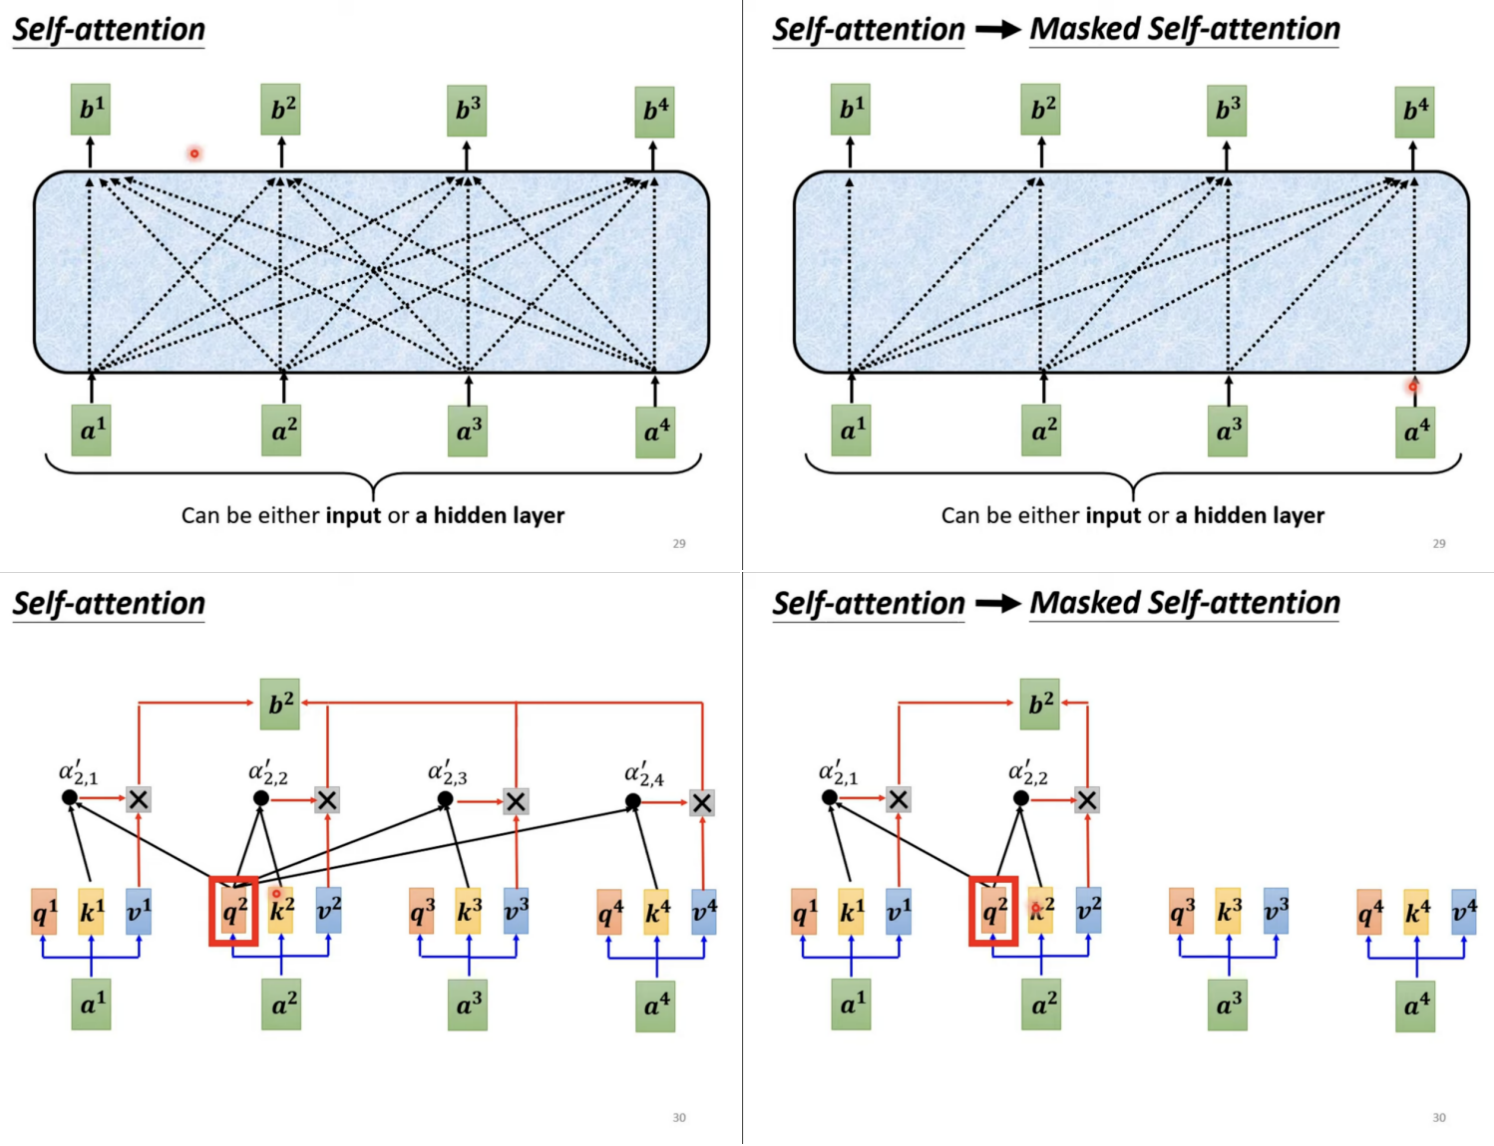
\includegraphics[width=0.9\linewidth]{figs/lec2/lec2.23.png}
  \caption{Self-Attention vs. Masked Self-Attention}
  \label{fig:Self-Attention vs. Masked Self-Attention}
\end{figure}


\clearpage

\subsubsection{Encoder-Decoder Attention(cross-attention)}


\subsubsection{Encoder-Decoder Attention (Cross-Attention)}

在 Cross-Attention 中:

\begin{figure}[htbp]
  \centering
  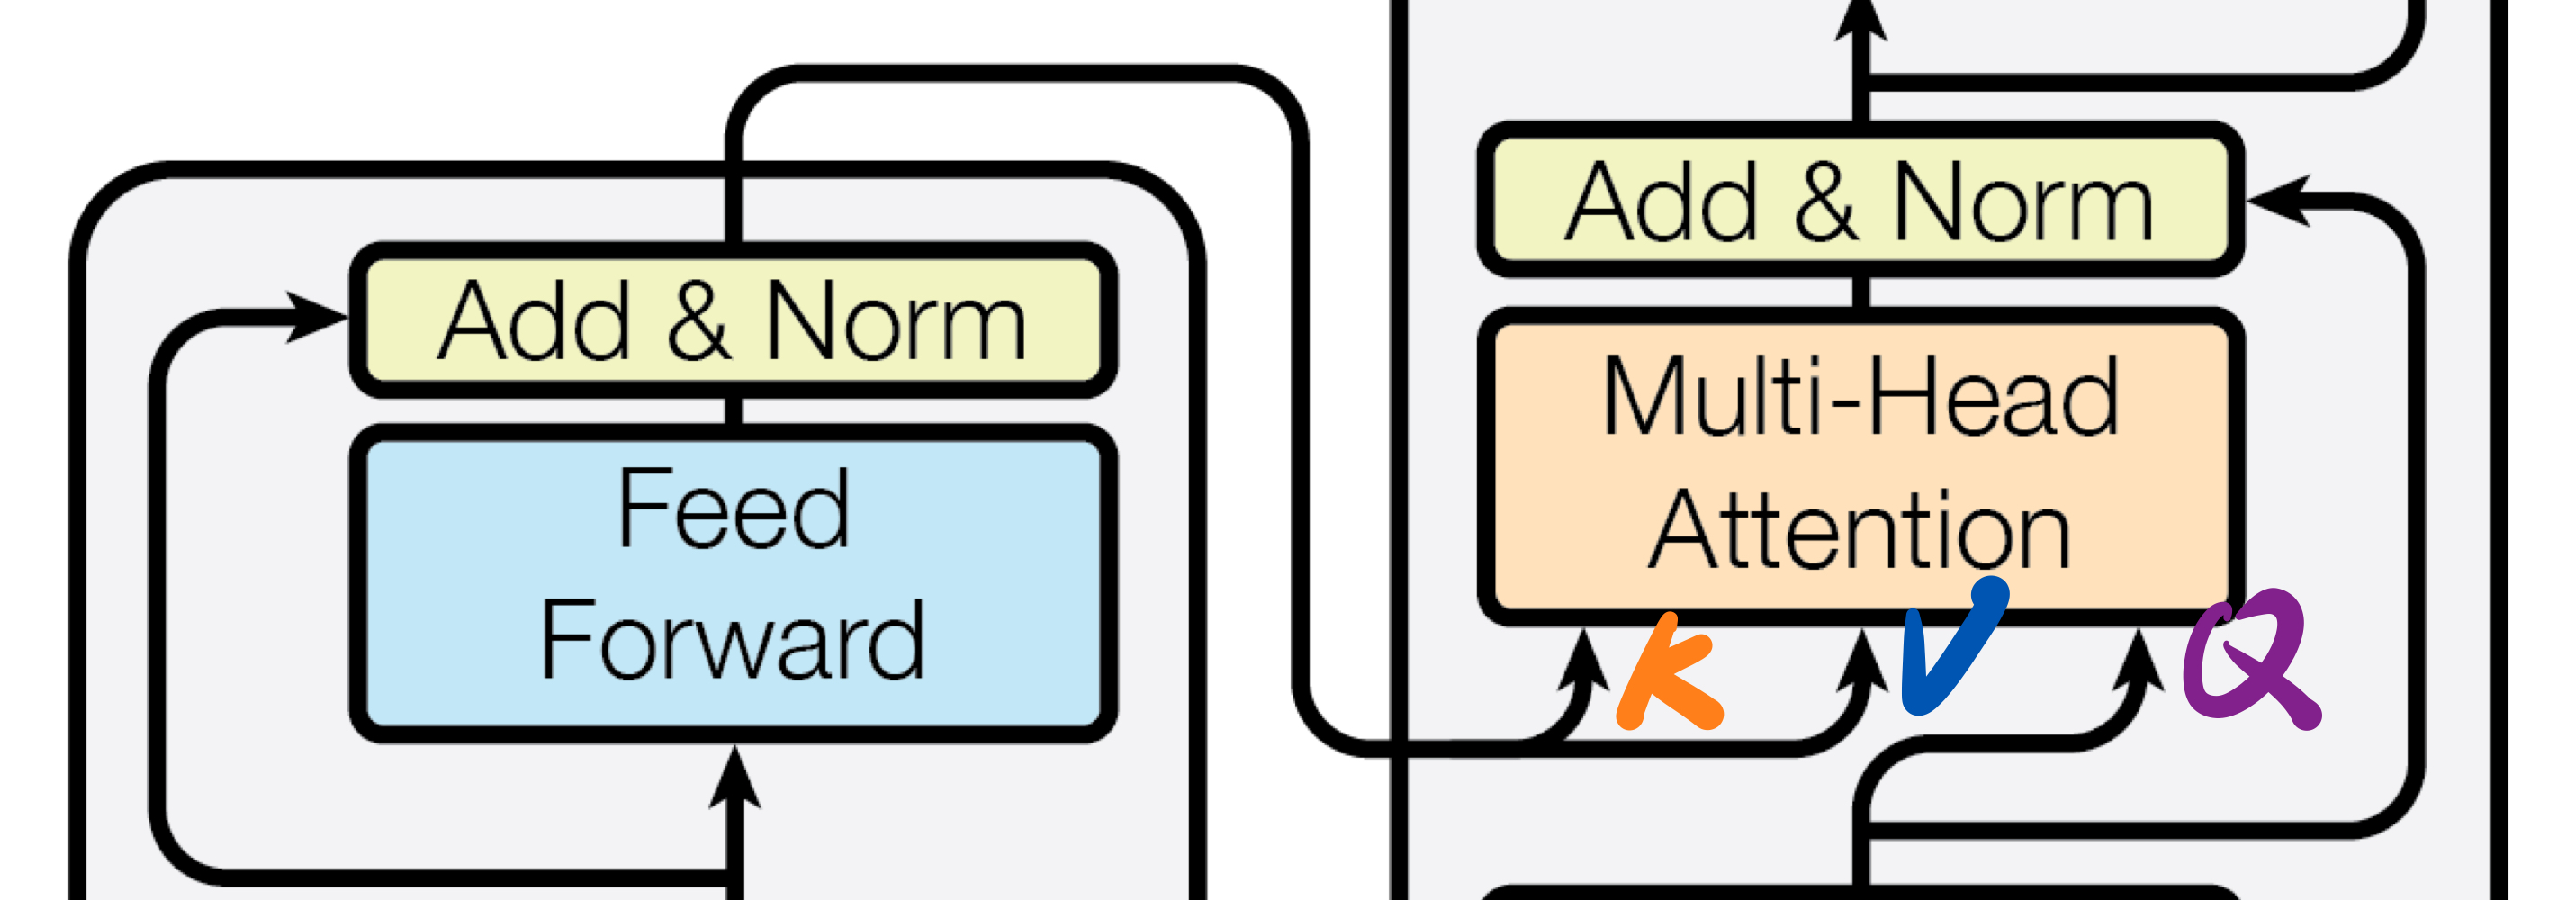
\includegraphics[width=0.6\linewidth]{figs/lec2/lec2.25.jpeg}
  \caption{Cross-Attention}
  \label{fig:Cross-Attention}
\end{figure}

\begin{itemize}
  \item {\color{qpurple}Query ($Q$)} 来自 Decoder 上一子层的输出(目标侧隐藏状态);
  \item {\color{orange}Key ($K$)} 与 {\color{zblue}Value ($V$)} 来自 Encoder 的最终输出(源侧隐藏状态)。
\end{itemize}
这样,Decoder 在生成目标 token 时,就能根据自身的解码状态(Query)去“检索”并选择性地利用 Encoder 编码的源序列信息(Key/Value)作为上下文,从而实现源-目标之间的信息交互。

Cross-Attention 的计算公式为:
\[
\text{CrossAttention}(Q, K, V) = \text{softmax}\left(\frac{QK^\mathsf{T}}{\sqrt{d_k}}\right)V
\]
这里的 $Q \in \mathbb{R}^{n_{\text{tgt}} \times d_k}$ 来自 Decoder,$K, V \in \mathbb{R}^{n_{\text{src}} \times d_k}$ 来自 Encoder。

\Remark{
\textbf{三种Attention的区别}
\begin{itemize}
  \item 在 {\color{tred}Self-Attention} 中,$Q, K, V$ 都来自同一个序列(Encoder 内部或 Decoder 内部)。
  \item 在 {\color{tred}Masked Self-Attention} 中(Decoder 第一子层),$Q, K, V$ 也来自 Decoder 内部,但会通过掩码屏蔽未来 token。
  \item 在 {\color{tred}Cross-Attention} 中,$Q$ 来自 Decoder,$K$ 和 $V$ 来自 Encoder,因此它连接了源语言和目标语言的信息。
\end{itemize}
}

这种设计保证了 Decoder 在生成每一个目标 token 时,都可以直接访问并利用 Encoder 编码好的全局源序列信息,而无需担心未来信息泄露问题。

\subsubsection{训练与推理差异}

在 Decoder 中,训练与推理的主要差异在于输入内容与生成方式:
\begin{itemize}
  \item \hyperref[def:teacher-forcing]{\textbf{训练(Teacher Forcing)}}:Decoder 输入完整的目标序列(右移一位作为输入),每个时间步都能看到真实的历史 token,通过 Masked Self-Attention 避免访问未来 token。
  \item \hyperref[def:auto-regressive]{\textbf{推理(Auto-regressive)}}:Decoder 每次仅输入已生成的 token(初始仅有 \texttt{<BOS>} 起始符),依次通过 Masked Self-Attention 生成下一个 token,直到生成结束符或达到最大长度。
\end{itemize}



\clearpage
\subsection{Output Projection \& Softmax}

Decoder 堆栈在每个时间步 $t$ 会输出一个隐藏向量 $\mathbf{h}_t \in \mathbb{R}^d$。为了将这个向量转化为具体的词,我们需要两步:

\MarginNote{
  \Definition{Logits}{
    神经网络最后一层在 Softmax 之前的{\color{tred}原始未归一化分数向量}。
    它的长度等于词汇表大小,每个分量对应一个词的打分,可能为正或负,总和不一定为 1。
    Softmax 会将 logits 转换为概率分布,用于生成下一个 token。
    \label{def:logits}
  }
}


\begin{enumerate}
  \item \textbf{线性映射(Linear Layer)}  
  使用一个全连接层将 $\mathbf{h}_t$ 投影到词汇表大小 $|V|$ 的 \hyperref[def:logits]{logits} 向量:
  \begin{equation}
  \mathbf{z}_t = \mathbf{h}_t W_o + \mathbf{b}_o,
  \end{equation}
  其中 $W_o \in \mathbb{R}^{d \times |V|}$,$\mathbf{b}_o \in \mathbb{R}^{|V|}$。  
  若词表大小为 $10{,}000$,则 $\mathbf{z}_t$ 的每个分量对应一个词的分数。
  
  \item \textbf{Softmax 概率归一化}  
  将 logits 转换为概率分布:
  \begin{equation}
  p_t^{(i)} = \frac{\exp(z_t^{(i)})}{\sum_{j=1}^{|V|} \exp(z_t^{(j)})},
  \end{equation}
  使得所有概率均为正且总和为 $1$。概率最大的词即为该时间步生成的输出。
\end{enumerate}

Softmax 的输出可以用于不同生成策略(如 $\arg\max$ 选取、随机采样或 Top-$k$ / nucleus 采样),从而得到下一个 token,并将其反馈到下一步解码。

\begin{figure}[htbp]
  \centering
  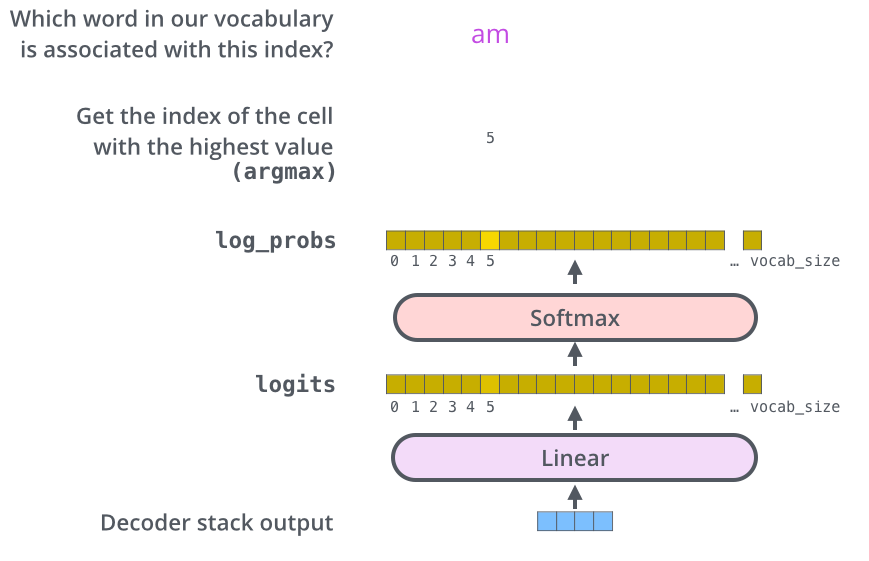
\includegraphics[width=0.9\linewidth]{figs/lec2/lec2.26.png}
  \caption{Linear + Softmax}
  \label{fig:Linear + Softmax}
\end{figure}









\clearpage
{\chaptoc\noindent\begin{minipage}[inner sep=0,outer sep=0]{0.9\linewidth}\section{Memory Accounting}\end{minipage}}

\subsection{Tensors Basics}
Tensors are the fundamental building block in PyTorch, used to store {\color{dblue}parameters, gradients, optimizer state, data, and activations}.

这里是Pytorch的tensors手册:\href{https://pytorch.org/docs/stable/tensors.html}{Pytorch docs on tensors}

创建tensor的方式有很多种,常用的有:
\begin{itemize}
    \item \texttt{torch.tensor([[1., 2, 3], [4, 5, 6]])} --- Create from data.
    \item \texttt{torch.zeros(4, 8)}, \texttt{torch.ones(4, 8)} --- Filled with zeros or ones.
    \item \texttt{torch.randn(4, 8)} --- Samples from $\mathcal{N}(0, 1)$.
    \item \texttt{torch.empty(4, 8)} --- Allocate without initialization (\texttt{torch.empty()} 只分配内存,不做初始化,所以得到的tensor是分配到的内存块里的原始数据).
\end{itemize}


\MarginNote{
\textbf{\texttt{nn.init.trunc\_normal\_}}  \\
将张量用截断正态分布 $\mathcal{N}(\mu, \sigma^2)$ 的值进行初始化,  
仅保留落在区间 $[a, b]$ 内的样本,其余会重新采样。  

该操作为原地(in-place)修改,会直接改变传入张量的内容。  
常用于网络权重初始化,以避免出现过大或过小的极端值。 
}

\Example{Custom initialization}
{
有时你会先分配一个未初始化的张量(例如 \texttt{torch.empty}),
因为你希望稍后用自定义逻辑来设置它的值。

例如,可以使用 \texttt{nn.init.trunc\_normal\_} 将张量按截断正态分布

$\mathcal{N}(\mu, \sigma^2)$ 初始化,限制值在区间 $[a, b]$ 内:

\texttt{nn.init.trunc\_normal\_(x, mean=0, std=1, a=-2, b=2)  \# 截断在 [-2, 2]}
}



\subsection{Tensors Memory}
\Remark{Almost everything (parameters, gradients, activations, optimizer states) are stored as floating point numbers.}

在学习不同Data Type之前我们需要回顾一下Sign bit, Exponent width和Significand precision三个基本概念。

\Definition{Sign Bit}{
浮点数最高位用于表示正负号,称为符号位(Sign bit)。  
符号位为 $0$ 表示正数,符号位为 $1$ 表示负数。
}

\Definition{Exponent Width}{
指数宽度(Exponent width)指浮点数用于存储指数的二进制位数。  
指数的位数决定了浮点数可表示的数值范围(范围越大,能表示的数越大或越小)。
}

\Definition{Significand Precision}{
有效数精度(Significand precision)指浮点数用于存储有效数字的二进制位数。  
有效位数越多,数值表示得越精确,计算结果的精度也越高。
}

\Definition{Floating-Point Representation}{
浮点数在计算机中的表示通常遵循 IEEE 754 标准,其通式为:
\[
(-1)^{\text{sign}} \times (1.\text{fraction})_2 \times 2^{\text{exponent} - \text{bias}}
\]
其中:
\begin{itemize}
    \item \textbf{sign} --- 符号位(Sign bit),决定数值正负。
    \item \textbf{fraction} --- 有效数字部分(Significand),用二进制表示。
    \item \textbf{exponent} --- 指数部分,决定数值的数量级。
    \item \textbf{bias} --- 指数偏移量(Bias),由指数位数决定,例如 8 位指数时 \(\text{bias} = 127\)。
\end{itemize}
}


\subsubsection{float32}
在 PyTorch 中,默认数据类型为 \texttt{\href{https://en.wikipedia.org/wiki/Single-precision_floating-point_format}{float32}}(单精度,fp32),在科学计算中,\texttt{float32} 是基准类型,也可在需要时使用双精度 \texttt{float64}。在深度学习中,数值精度要求相对宽松。

\MarginNote{
\Example{内存计算示例}{
\texttt{
x = torch.zeros(4, 8)\\
assert x.dtype == torch.float32 \# 默认类型\\
assert x.numel() == 4 * 8 \# 元素数量\\
assert x.element\_size() == 4 \# float32 占 4 字节\\
assert get\_memory\_usage(x) == 4 * 8 * 4 \# 128 字节
}
}
}

\Remark{
\textbf{张量的内存占用由以下两部分决定:}
\begin{enumerate}
    \item \textbf{元素数量}(\texttt{numel}):张量中值的总个数。
    \item \textbf{数据类型大小}(\texttt{element\_size}):每个元素占用的字节数。
\end{enumerate}
}


\begin{figure}[htbp]
  \centering
  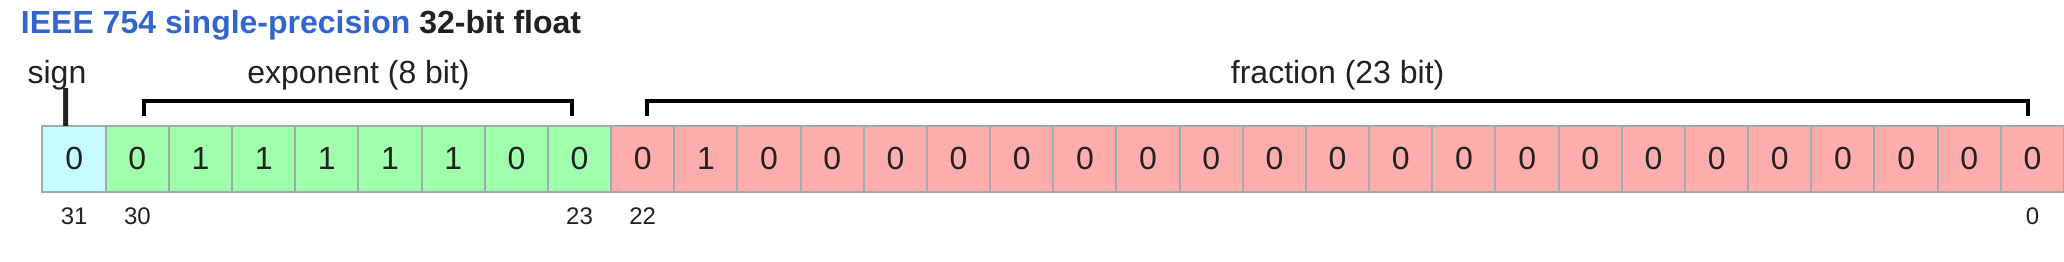
\includegraphics[width=0.9\linewidth]{figs/lec2/lec2.27.png}
  \caption{float32 内存结构示意图}
  \label{fig:float32 内存结构示意图}
\end{figure}



The IEEE 754 standard specifies a binary32 as having:
\begin{itemize}
    \item Sign bit: 1 bit
    \item Exponent width: 8 bits
    \item Significand precision: 24 bits (23 explicitly stored)
\end{itemize} 

\MarginImageWithNote
  {figs/lec2/lec2.28.jpeg}
  {\captionof{figure}{FP32的一些特性}}
  {图源本人的CS61C的Study Sheet}



\clearpage
\subsubsection{float16}

\texttt{float16}(半精度,fp16)将每个浮点数的内存占用从 \texttt{float32} 的 4 字节减少到 2 字节,可以显著节省显存。

\begin{figure}[htbp]
  \centering
  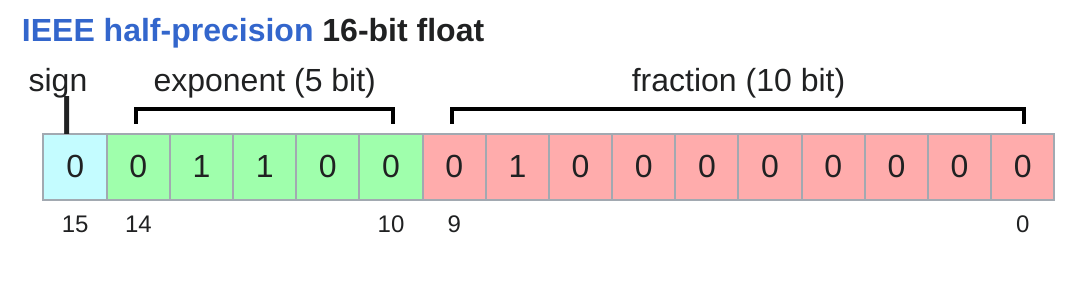
\includegraphics[width=0.9\linewidth]{figs/lec2/lec2.29.png}
  \caption{float16 内存结构示意图}
  \label{fig:float16 内存结构示意图}
\end{figure}


\MarginNote{
\Definition{Overflow and Underflow}{
\textbf{溢出(Overflow)}是指计算结果的绝对值超过了该数据类型所能表示的最大有限值。  
当发生溢出时,结果会被表示为 $+\infty$ 或 $-\infty$(即 IEEE 754 的 Infinity)。

例如,在 \texttt{float32} 中:
\[
x = 1\times 10^{40} \quad \Rightarrow \quad x \to +\infty
\]

\textbf{下溢(Underflow)}是指计算结果的绝对值小于该数据类型所能表示的最小正数(包括次正规数范围)。  
当发生下溢时,结果可能会变为 \texttt{0}(flush-to-zero)或以较低精度的次正规数表示。

例如,在 \texttt{float16} 中:
\[
x = 1\times 10^{-8} \quad \Rightarrow \quad x \to 0
\]
}
}

The IEEE 754 standard specifies a binary16 as having the following format:
\begin{itemize}
  \item Sign bit: 1 bit
  \item Exponent width: 5 bits
  \item Significand precision: 11 bits (10 explicitly stored)
\end{itemize} 

\texttt{float16} 的动态范围较差,容易发生下溢(Underflow)。


\subsubsection{bfloat16}

Google Brain 在 2018 年提出了 \texttt{bfloat16}(Brain Floating Point),
目的是缓解 \texttt{float16} 动态范围过小的问题。
\texttt{bfloat16} 与 \texttt{float16} 占用相同内存(2 字节),
但其动态范围与 \texttt{float32} 相同!
代价是精度(有效位数)更低,不过在深度学习中通常无碍。

\begin{figure}[htbp]
  \centering
  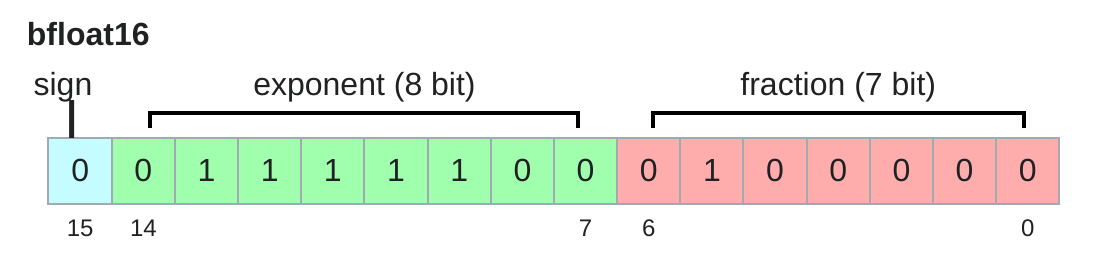
\includegraphics[width=0.9\linewidth]{figs/lec2/lec2.30.png}
  \caption{float16 内存结构示意图}
  \label{fig:float16 内存结构示意图}
\end{figure}

bfloat16 has the following format:
\begin{itemize}
  \item Sign bit: 1 bit
  \item Exponent width: 8 bits
  \item Significand precision: 8 bits (7 explicitly stored, with an implicit leading bit), as opposed to 24 bits in a classical single-precision floating-point format
\end{itemize}

\MarginImageWithNote
  {figs/lec2/lec2.31.png}
  {\captionof{figure}{三种Data Type的性能比较}}


\clearpage
\subsubsection{fp8}
2022 年,FP8 格式被标准化,主要是为机器学习工作负载优化。
NVIDIA H100 支持两种 FP8 变体:

\textbf{E4M3}:4 位指数,3 位尾数,有效范围约为 $[-448, 448]$,精度较高、范围窄。

\textbf{E5M2}:5 位指数,2 位尾数,有效范围约为 $[-57344, 57344]$,范围广、精度低。

\begin{figure}[htbp]
  \centering
  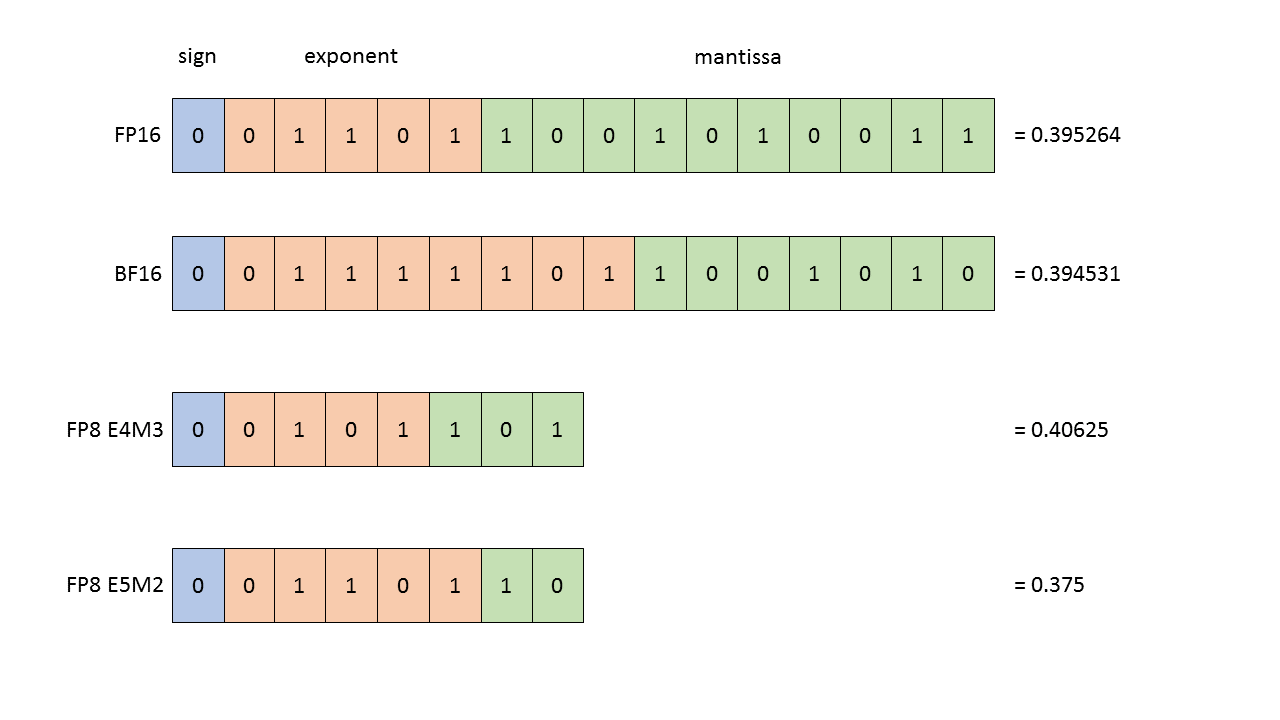
\includegraphics[width=0.9\linewidth]{figs/lec2/lec2.32.png}
  \caption{fp8 内存结构示意图}
  \label{fig:fp8 内存结构示意图}
\end{figure}

\Remark{
训练时:
\begin{itemize}
    \item 使用 \texttt{float32} 训练稳定,但显存占用大。
    \item 直接使用 \texttt{fp8}、\texttt{float16} 或 \texttt{bfloat16} 训练,风险较高,易数值不稳定。
    \item 解决方案:混合精度训练(\texttt{mixed\_precision\_training})。
\end{itemize}
}

\begin{table}[h]
\centering
\renewcommand{\arraystretch}{1.3}
\begin{tabular}{l l l l l}
\hline
\textbf{Property} & \textbf{fp32} & \textbf{fp16} & \textbf{bfloat16} & \textbf{fp8 (E4M3 / E5M2)} \\
\hline
Sign bit & 1 & 1 & 1 & 1 \\
Exponent width & 8 & 5 & 8 & 4 / 5 \\
Significand precision & 23 bits & 10 bits & 7 bits & 3 bits / 2 bits \\
Largest finite value & $3.4\times 10^{38}$ & $6.55\times 10^{4}$ & $3.4\times 10^{38}$ & $\approx 448$ / $\approx 5.73\times 10^{4}$ \\
Smallest positive normal & $1.17\times 10^{-38}$ & $6.10\times 10^{-5}$ & $1.17\times 10^{-38}$ & $\approx 2^{-6}$ / $\approx 2^{-14}$ \\
Element size & 4 bytes & 2 bytes & 2 bytes & 1 byte \\
Supports Infinity / NaN & Yes & Yes & Yes & Yes \\
Underflow risk & Very low & High & Very low & Very high \\
\hline
\end{tabular}
\caption{Comparison of common floating-point formats for deep learning}
\label{tab:fp_all_compare}
\end{table}

\clearpage
\subsection{Mixed Precision Training \href{https://arxiv.org/pdf/1710.03740.pdf}{[Micikevicius et al., 2017]}}

\paragraph{技术背景}~{}
\begin{itemize}
    \item 深度学习模型复杂化与数据集规模不断增长,显著增加显存和计算资源需求。
    \item 使用低精度(如 FP16)可减少显存占用并提升计算吞吐率,在新 GPU上可带来 2--8 倍算力提升。
    \item 直接用 FP16 训练会因数值范围有限而引发训练不稳定或精度下降。
\end{itemize}


\MarginImageWithNote
  {figs/lec2/lec2.34.png}
  {\captionof{figure}{FP32和FP16的性能对比}}
  {
\footnotesize
神经网络训练与推理的性能瓶颈主要有三类:
\begin{itemize}[leftmargin=0.5em]
    \item 算术带宽(Arithmetic Bandwidth)
    \item 内存带宽(Memory Bandwidth)
    \item 延迟(Latency)
\end{itemize}
采用低精度可缓解前两者:
\begin{itemize}[leftmargin=0.5em]
    \item 更少比特存储,降低内存带宽压力
    \item 高吞吐低精度运算,减少算术时间
\end{itemize}
例如在新一代 GPU 中,半精度吞吐率可达单精度的 2--8 倍,
且训练显存需求也随之降低。
}


\begin{figure}[htbp]
  \centering
  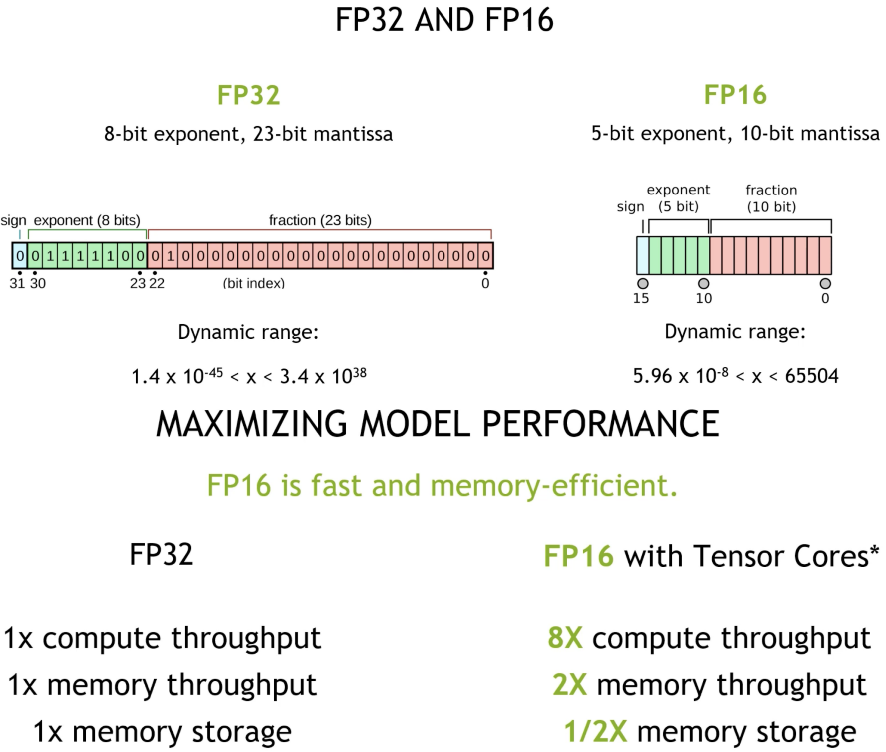
\includegraphics[width=0.9\linewidth]{figs/lec2/lec2.33.png}
  \caption{FP32 vs. FP16}
  \label{fig:FP32 vs. FP16}
\end{figure}

\Remark{Mixed Precision Training 的目标是在缓解内存压力、提升计算吞吐的同时保持模型精度,
通过在关键环节保留高精度、非关键环节使用低精度,从而兼顾性能与准确性。}


\paragraph{核心挑战——FP16的低精度和Narrow dynamic range:}~{}
\begin{itemize}
    \item \textbf{精度损失}:多次累加 FP16 乘积时精度损失显著,尤其是矩阵乘法、大规模求和等运算中。
    \item \textbf{Narrow dynamic range}:FP16低精度可能导致梯度更新不稳定,梯度分布中大量小值发生 underflow,影响模型收敛。
\end{itemize}

\paragraph{技术路径}~{}

\textbf{{\color{tred}Single-precision master weights and updates, loss-scaling, and accumulating FP16 products into FP32}}


\begin{enumerate}
    \item \textbf{FP32 Master Copy of Weights}:在前向与反向传播中,权重、激活、梯度均用 FP16 存储和计算;但在优化器更新时,维护一份 FP32 主副本来累积梯度并更新权重,再将其转换为 FP16 用于下一轮迭代。这可以避免更新量过小而在 FP16 下舍入为零的问题。

    \item \textbf{Loss Scaling}:由于梯度值分布中大量数值很小,容易在 FP16 下发生下溢(underflow)而变成零,训练会发散。通过在反向传播前将损失乘以一个常数因子(如 $8$、$128$),可同步放大所有梯度,使它们落入 FP16 可表示范围;在更新前再除回该因子,保持与 FP32 训练一致的更新幅度。
    
    \item \textbf{Arithmetic Precision}:对向量点积、卷积等操作,输入用 FP16 存储,但乘法先转换到 FP32 精度计算,并在 FP32 累加器中累积结果,最后再存回 FP16;大规模求和(如 Batch Norm 统计量、Softmax 归一化)也在 FP32 下进行;逐元素操作则可直接用 FP16。
\end{enumerate}


\subparagraph{FP32 Master Copy of Weights}~{}

\begin{figure}[htbp]
  \centering
  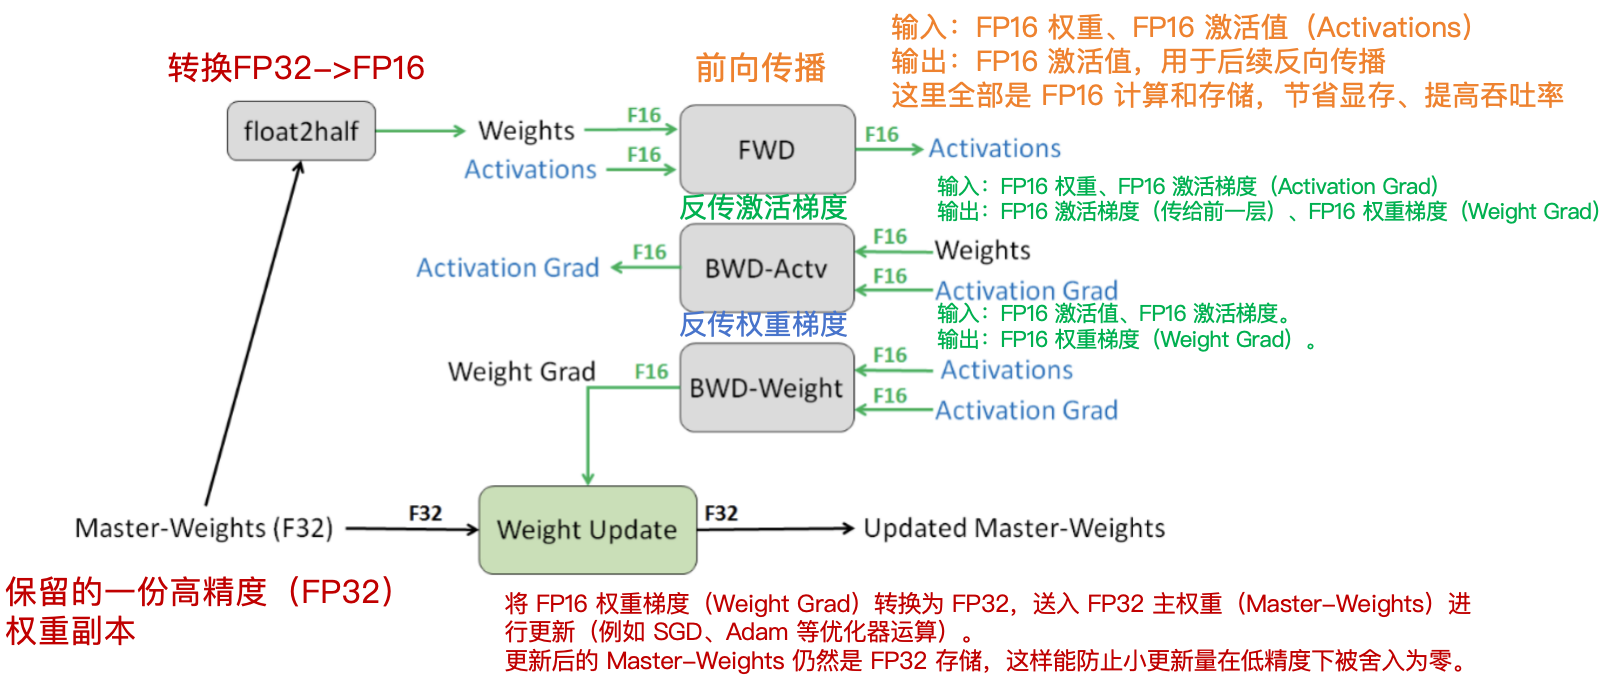
\includegraphics[width=1.1\linewidth]{figs/lec2/lec2.36.png}
  \caption{Mixed precision training iteration for a layer.}
  \label{Mixed precision training iteration for a layer.}
\end{figure}

\subparagraph{Loss Scaling}~{}


\MarginImageWithNote
  {figs/lec2/lec2.38.png}
  {\captionof{figure}{Multibox SSD 网络训练时激活梯度的分布直方图}}
  {
  \footnotesize
  横轴为梯度大小的 $\log_2$,纵轴为该范围梯度占所有梯度的百分比,最左侧单独的柱表示梯度为 0 的比例。

  \textbf{关键标记:}
  \begin{itemize}[leftmargin=0.5em]
      \item \textcolor{red}{红线}:FP16 norms($\approx 2^{-24}$),左侧梯度在 FP16 下直接变为 0
      \item \textcolor{blue}{蓝线}:FP16 denorms下限($\approx 2^{-14}$),范围内精度显著下降
      \item \textcolor{black}{黑色箭头}:FP16 的整体可表示范围上限
  \end{itemize}

  直接用 FP16 存储梯度时,会严重 \emph{underflow},约 $67\%$ 的梯度值为零。
  因此需要在反向传播中采用 \textbf{Loss Scaling} 来缓解。
  }


\begin{figure}[htbp]
  \centering
  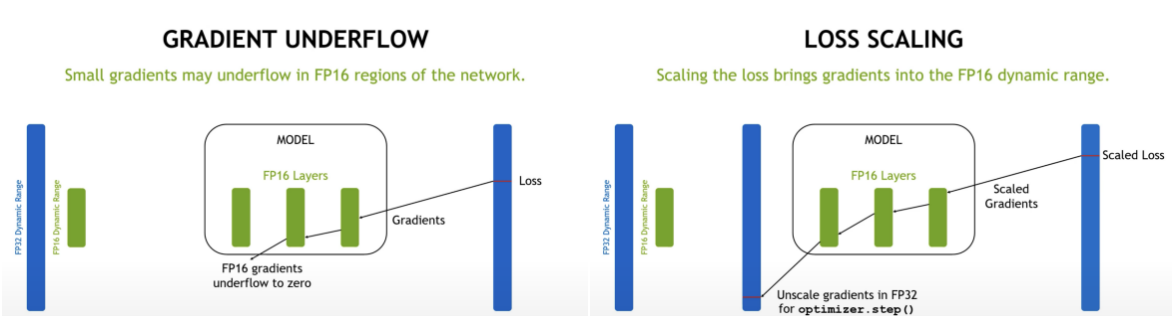
\includegraphics[width=0.8\linewidth]{figs/lec2/lec2.37.png}
  \caption{Loss Scaling}
\label{Loss Scaling}
\end{figure}


\clearpage
\subparagraph{Arithmetic Precision}~{}

在混合精度训练中,现代 GPU(如 Volta/Turing/Ampere 的 Tensor Cores)常采用
\textbf{FP16 inputs、FP32 multiply-accumulate (MAC)} 的策略,以兼顾吞吐与精度:

\begin{itemize}[leftmargin=1em]
    \item \textbf{存储与搬运阶段}:\textit{weights} 与 \textit{activations} 在显存和寄存器中以 FP16 存储,降低显存占用与内存带宽压力;
    \item \textbf{硬件执行阶段(Tensor Core 内部)}:
    \begin{enumerate}[label= (\alph*), leftmargin=1.5em]
        \item 每对 FP16 操作数在进入运算管线前,由硬件逻辑\emph{自动}扩展(cast)为 FP32;
        \item 在 FP32 精度下完成乘法(multiply);
        \item 乘积直接送入 FP32 累加器(accumulator)进行加法累积(accumulate),保留 23 位尾数精度;
    \end{enumerate}
    \item \textbf{输出阶段}:累积完成后,可选择保持 FP32(精度敏感路径)或压缩回 FP16(节省存储与带宽)。
\end{itemize}

以矩阵乘法为例:
\[
C_{ij} = \sum_{k=1}^n 
\mathrm{cast}(A_{ik})_{\mathrm{fp16}\to\mathrm{fp32}}
\times
\mathrm{cast}(B_{kj})_{\mathrm{fp16}\to\mathrm{fp32}}
\ \xrightarrow[\text{FP32 multiply}]{\text{Tensor Core}}\ 
\mathrm{product}_{\mathrm{fp32}}
\ \xrightarrow{\text{FP32 accumulate}}\ 
\mathrm{accumulator}_{\mathrm{fp32}}
\]


其中 $A_{ik}$ 与 $B_{kj}$ 虽以 FP16 存储,但在进入 Tensor Core 计算管线时即被扩展到 FP32,
整个 multiply-accumulate 流程均在硬件内部的 FP32 数据通路上完成。

这种方式结合了:
\begin{itemize}[leftmargin=1em]
    \item \textbf{FP16 存储通路}:降低显存和寄存器压力,提升内存带宽与并行度;
    \item \textbf{FP32 计算通路}:在乘法与累加阶段保留高精度,有效抑制数值漂移。
\end{itemize}

在该模式下,V100 的矩阵乘法吞吐量可达 FP32 的 8 倍(125 TFLOPs),
A100 更可达 16 倍(312 TFLOPs)。

\begin{figure}[htbp]
  \centering
  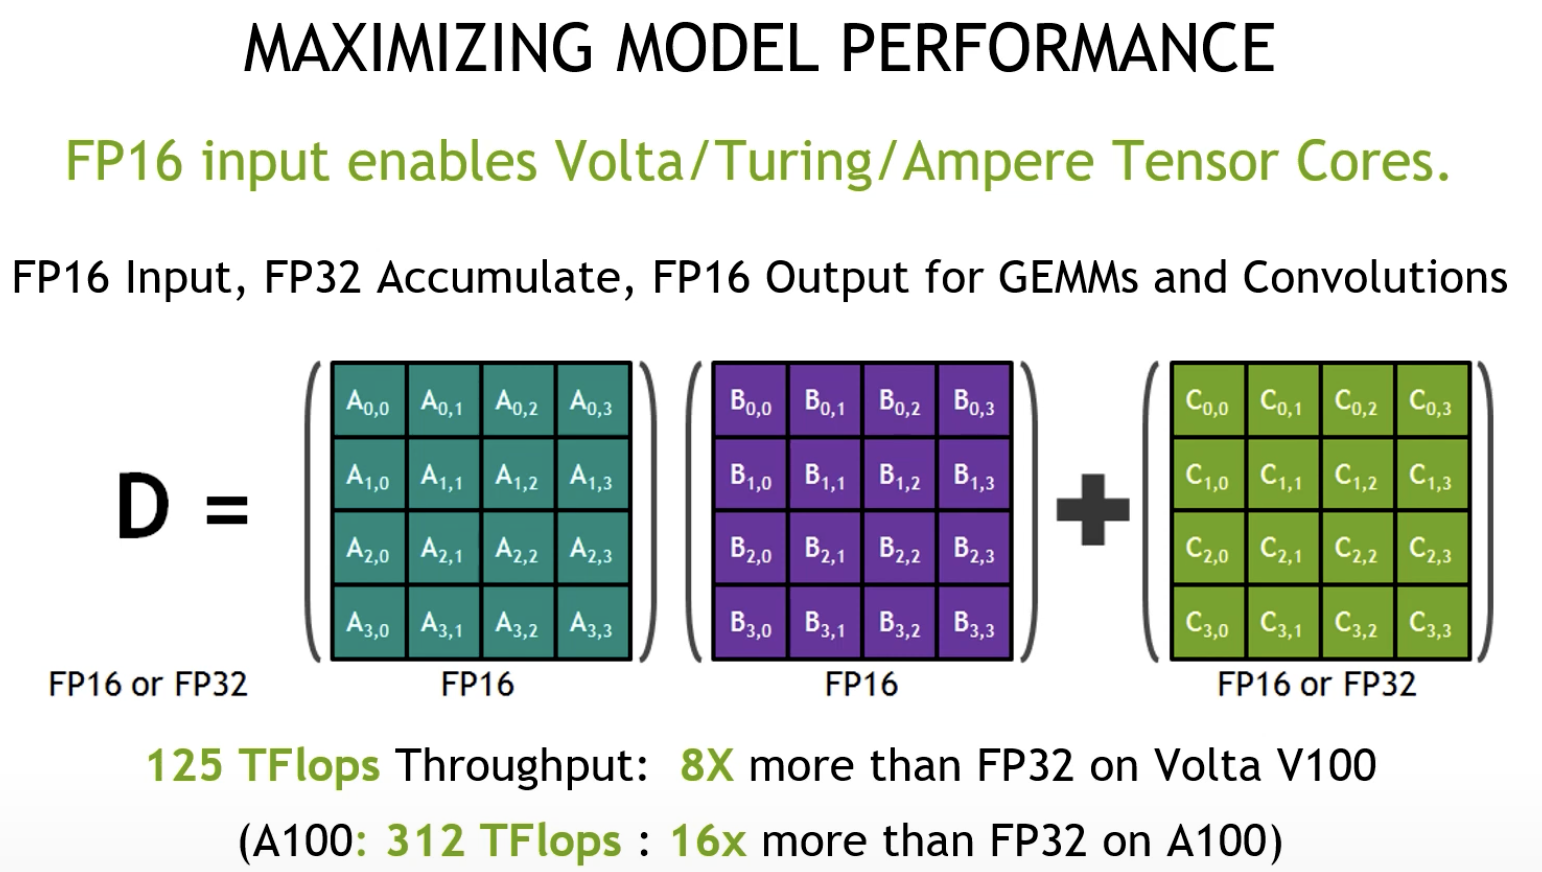
\includegraphics[width=0.8\linewidth]{figs/lec2/lec2.35.png}
  \caption{
    FP16 存储、Tensor Core 内部 FP32 multiply-accumulate 的数据流示意。
    输入存储为低精度以提高吞吐,计算与累加在硬件内部保持高精度以确保数值稳定性。
  }
\label{fig:arithmetic_precision}
\end{figure}


\subparagraph{AMP: Automatic Mixed Precision}~{}

\MarginImageWithNote
  {figs/lec2/lec2.39.png}
  {\captionof{figure}{AMP code example}}




\begin{itemize}
    \item PyTorch 提供了 \href{https://pytorch.org/docs/stable/amp.html}{Automatic Mixed Precision (AMP)} 库,
    可自动在 \texttt{float32} 与低精度之间切换。
    \item NVIDIA 的 \href{https://docs.nvidia.com/deeplearning/performance/mixed-precision-training/}{性能优化指南}
    和 \href{https://docs.nvidia.com/deeplearning/transformer-engine/user-guide/}{Transformer Engine}
    支持在线性层中使用 FP8,并在训练中广泛使用.
\end{itemize}



\clearpage
{\chaptoc\noindent\begin{minipage}[inner sep=0,outer sep=0]{0.9\linewidth}\section{Compute Accounting}\end{minipage}}

\subsection{Tensors On Gpus}~{}

默认情况下,PyTorch 创建的张量会存储在 CPU 内存中:

为了利用 GPU 的大规模并行计算能力,需要将张量移动到 GPU 内存。

\begin{lstlisting}[language=Python]
    # 默认创建在 CPU
    x = torch.zeros(32, 32)
    assert x.device == torch.device("cpu")

    if torch.cuda.is_available():
        # GPU 属性
        for i in range(torch.cuda.device_count()):
            print(torch.cuda.get_device_properties(i))

        mem0 = torch.cuda.memory_allocated()

        # CPU -> GPU0
        y = x.to("cuda:0")
        assert y.device == torch.device("cuda", 0)

        # 或者直接在 GPU 创建
        z = torch.zeros(32, 32, device="cuda:0")
\end{lstlisting}

\begin{figure}[htbp]
  \centering
  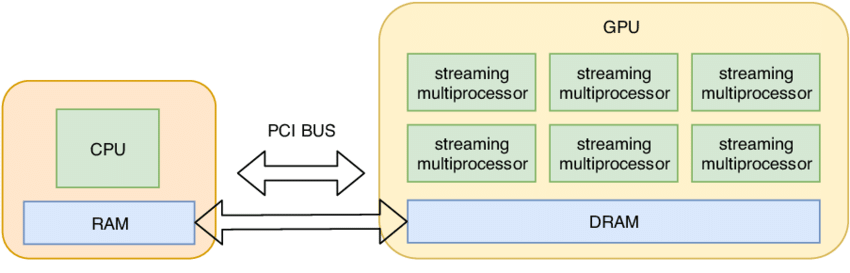
\includegraphics[width=0.9\linewidth]{figs/lec2/lec2.40.png}
  \caption{Move tensor from CPU to GPUs}
\end{figure}

\par

\begin{itemize}
    \item 检查 GPU 内存使用情况:可以使用 \texttt{torch.cuda.memory\_allocated()} 查看当前 GPU 上已分配的内存。
    \item 释放 GPU 内存:使用 \texttt{torch.cuda.empty\_cache()} 可以释放未使用的 GPU 内存,但不会影响当前已分配的张量。
\end{itemize}



\clearpage
\subsection{Tensor Operations}

\subsubsection{Tensor Storage}

PyTorch 张量(Tensor)本质上是指向已分配内存的指针,外加描述如何访问任意元素的元数据(metadata)。

\begin{figure}[htbp]
  \centering
  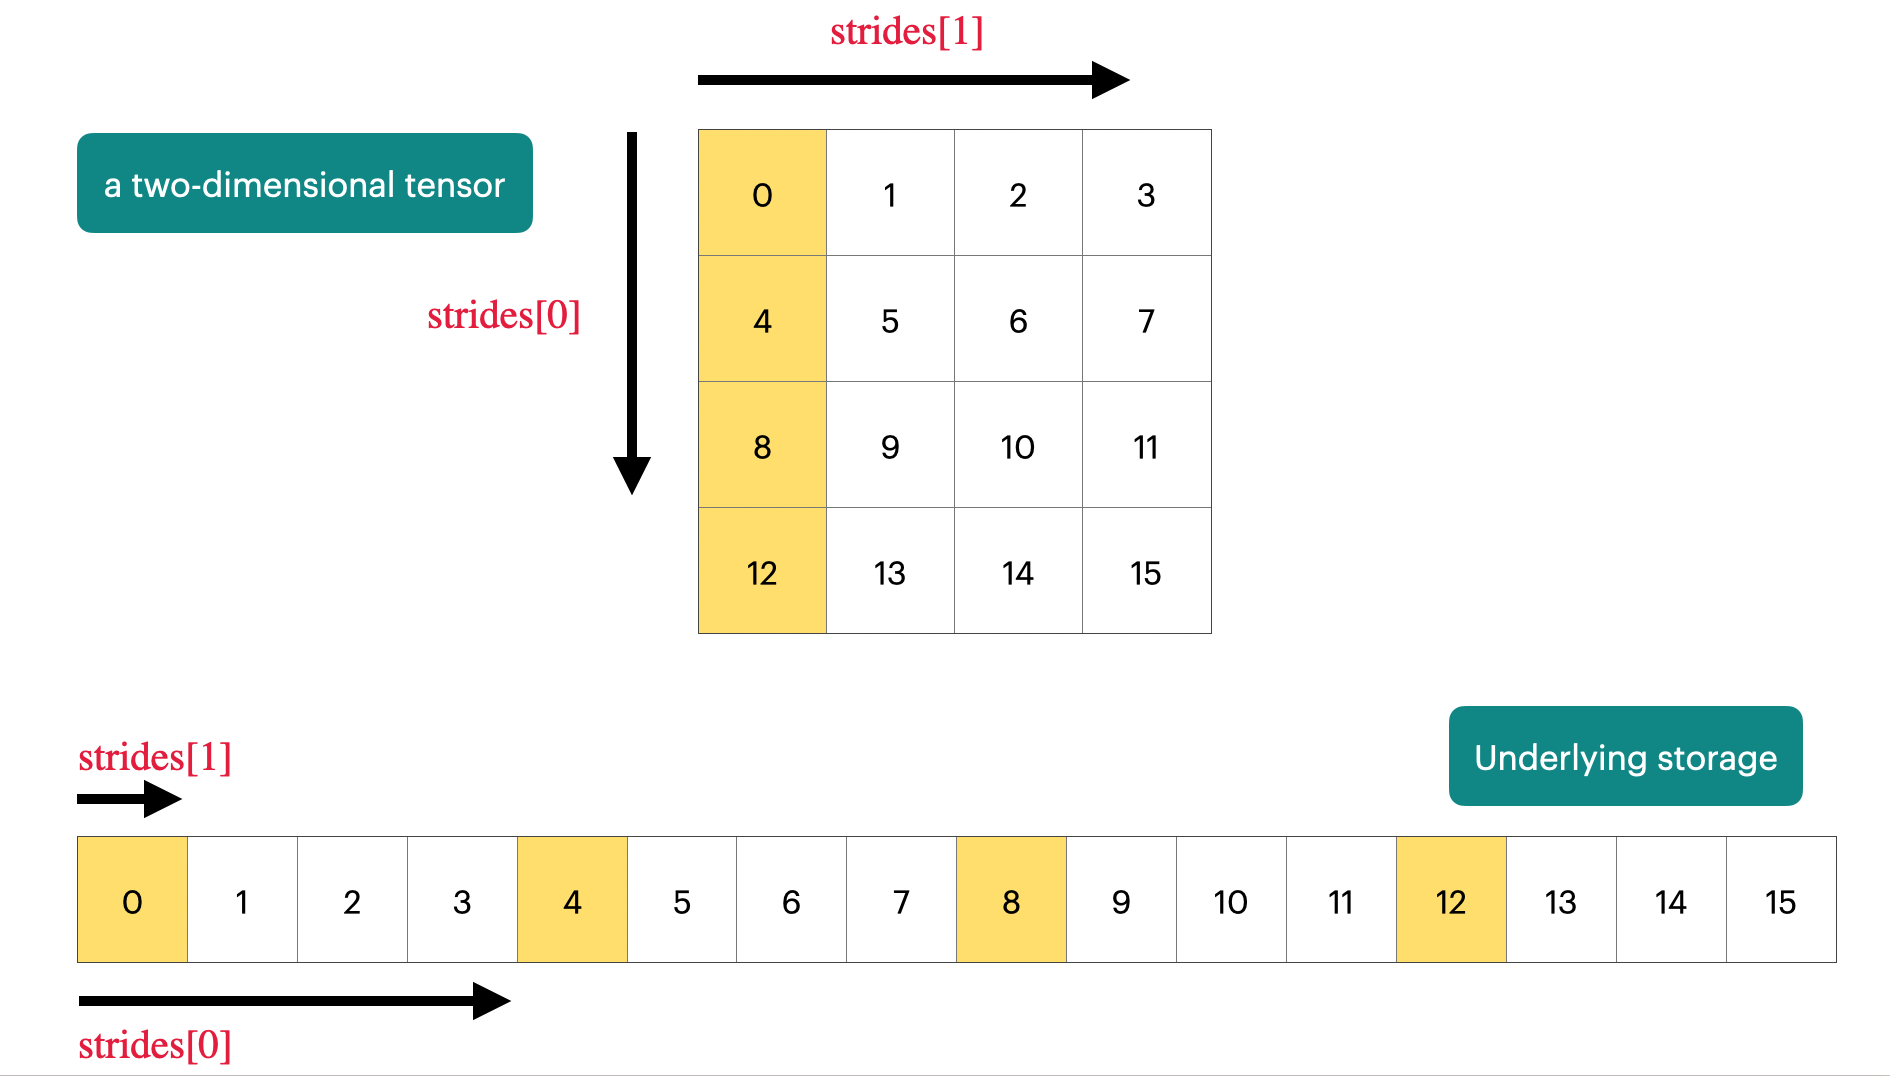
\includegraphics[width=0.9\linewidth]{figs/lec2/lec2.41.png}
  \caption{Tensor Storage}
  \label{fig:Tensor Storage}
\end{figure}  

\begin{lstlisting}[language=Python]

# 到下一行(dim 0)需要跳过 4 个元素
assert x.stride(0) == 4

# 到下一列(dim 1)需要跳过 1 个元素
assert x.stride(1) == 1

# 计算元素 (r, c) 的存储索引
r, c = 1, 2
index = r * x.stride(0) + c * x.stride(1)
assert index == 6
\end{lstlisting}

\subsubsection{Tensor Slicing}

很多操作仅仅提供张量的不同\textbf{视图(view)},不会复制数据,因此一个张量的修改会影响另一个。
\MarginNote{
{\color{qpurple}\textbf{\texttt{torch.transpose(input, dim0, dim1)}}}  

交换张量的两个维度(\texttt{dim0} 与 \texttt{dim1})。  
\vspace{0.5em}

\textbf{例 1(二维矩阵)}:  
输入形状 $(2, 3)$,交换 0、1 轴:  
\[
\begin{bmatrix}
1 & 2 & 3 \\
4 & 5 & 6
\end{bmatrix}
\to
\begin{bmatrix}
1 & 4 \\
2 & 5 \\
3 & 6
\end{bmatrix}
\]  

\textbf{例 2(三维张量)}:  
输入形状 $(2, 3, 4)$,交换第 1、2 轴:  
原索引 $(b, h, w)$ 变为 $(b, w, h)$。  
假设 $x.shape = (2, 3, 4)$:  
\[
x.transpose(1, 2) \ \Rightarrow\ \text{shape} = (2, 4, 3)
\]  

\textbf{共享内存}:  
若输入是 \emph{strided tensor}(密集张量),结果与输入共享底层存储,因此修改其中一个会影响另一个。  
\vspace{0.3em}
若是稀疏张量(sparse tensor),是否共享取决于存储布局(CSR、CSC 等)。  
}

\MarginNote{
\fontsize{10pt}{12pt}\selectfont
\textbf{非连续 (non-contiguous) 张量}:
PyTorch 张量底层由 \emph{一维内存块 (storage)} 加 \emph{步幅 (stride)} 决定访问方式。
某些操作(如 \texttt{transpose}、\texttt{permute})只会改变 stride,而不移动内存。
这样虽然逻辑顺序正确,但物理内存不再按行优先紧密排列。

\textbf{影响}:\texttt{.view()} 只能在连续 (contiguous) 内存上使用,非连续张量会报错。

\textbf{解决}:用 \texttt{.contiguous()} 重新拷贝数据,使其在内存中连续存储,再 \texttt{.view()}。
}



\begin{lstlisting}[language=Python]
x = torch.tensor([[1., 2, 3], [4, 5, 6]])

# 获取第 0 行
y = x[0]
% assert torch.equal(y, torch.tensor([1., 2, 3]))
% assert same_storage(x, y)

# 获取第 1 列
y = x[:, 1]
assert torch.equal(y, torch.tensor([2, 5]))
assert same_storage(x, y)

# 视作 3x2 矩阵
y = x.view(3, 2)
assert torch.equal(y, torch.tensor([[1, 2], [3, 4], [5, 6]]))
assert same_storage(x, y)

# 转置
y = x.transpose(1, 0)
assert torch.equal(y, torch.tensor([[1, 4], [2, 5], [3, 6]]))
assert same_storage(x, y)

# 修改 x 会影响 y
x[0][0] = 100
assert y[0][0] == 100

# 非连续张量视图无法直接 .view()
y = x.transpose(1, 0)
assert not y.is_contiguous()
try:
    y.view(2, 3)
except RuntimeError as e:
    assert "view size is not compatible" in str(e)

# 先转为连续再 .view()
y = x.transpose(1, 0).contiguous().view(2, 3)
assert not same_storage(x, y)
\end{lstlisting}
\vspace{-1em}



\subsubsection{Elementwise Operations}

逐元素运算会对张量的每个元素应用相同的操作,并返回相同形状的\textbf{新张量}。

\begin{lstlisting}[language=Python]
x = torch.tensor([1, 4, 9])
assert torch.equal(x.pow(2), torch.tensor([1, 16, 81]))
assert torch.equal(x.sqrt(), torch.tensor([1, 2, 3]))
assert torch.equal(x.rsqrt(), torch.tensor([1, 1/2, 1/3])) # i -> 1/sqrt(x_i)
assert torch.equal(x + x, torch.tensor([2, 8, 18]))
assert torch.equal(x * 2, torch.tensor([2, 8, 18]))
assert torch.equal(x / 0.5, torch.tensor([2, 8, 18]))

# 上三角矩阵
x = torch.ones(3, 3).triu()
assert torch.equal(x, torch.tensor([
    [1, 1, 1],
    [0, 1, 1],
    [0, 0, 1],
]))
\end{lstlisting}

\MarginNote{
{\color{qpurple}\textbf{\texttt{torch.triu(input, diagonal=0)}}}  

返回矩阵(2D 张量)或矩阵批次的\textbf{上三角部分},其余元素置为 $0$。  

\vspace{0.3em}
\textbf{默认}:\texttt{diagonal=0} 保留主对角线及其上方元素。  
\[
\begin{bmatrix}
1 & 2 & 3 \\
4 & 5 & 6 \\
7 & 8 & 9
\end{bmatrix}
\ \xrightarrow{\ \texttt{triu}\ }\ 
\begin{bmatrix}
1 & 2 & 3 \\
0 & 5 & 6 \\
0 & 0 & 9
\end{bmatrix}
\]  

\vspace{0.3em}
\textbf{参数 diagonal}:  
\begin{itemize}
    \item \texttt{0}:主对角线及以上  
    \item \texttt{>0}:排除更靠上的对角线(向上移)  
    \item \texttt{<0}:包含主对角线下方的更多元素(向下移)
\end{itemize}  

例如:
\[
\texttt{triu(A, 1)} \Rightarrow
\begin{bmatrix}
0 & 2 & 3 \\
0 & 0 & 6 \\
0 & 0 & 0
\end{bmatrix}
\]  
}

\begin{itemize}[leftmargin=1.5em]
    \item 常用在数学变换(幂、开方、加减乘除等)。
    \item \verb|triu| 可用于生成因果注意力掩码。
\end{itemize}


\subsubsection{Matrix Multiplication}

深度学习的核心操作之一是矩阵乘法(matmul)。

\begin{lstlisting}[language=Python]
# 基本矩阵乘法
x = torch.ones(16, 32)
w = torch.ones(32, 2)
y = x @ w
assert y.size() == torch.Size([16, 2])

# 批量矩阵乘法
x = torch.ones(4, 8, 16, 32)
w = torch.ones(32, 2)
y = x @ w
assert y.size() == torch.Size([4, 8, 16, 2])
\end{lstlisting}

\MarginNote{
{\color{qpurple}\textbf{\texttt{x @ w} 批量矩阵乘法}}  

输入:  
\texttt{x.shape = [4, 8, 16, 32]}  
\texttt{w.shape = [32, 2]}  

\vspace{0.3em}
\textbf{规则}:  
\begin{itemize}
  \item 前两维 \texttt{[4, 8]} 作为批次维度保留  
  \item 每个 \texttt{[16, 32]} 子矩阵与 \texttt{[32, 2]} 相乘  
  \item 得到 \texttt{[16, 2]},再拼回批次维度 $\Rightarrow$ \texttt{[4, 8, 16, 2]}
\end{itemize}

\vspace{0.3em}
In this case, we iterate over values of the first 2 dimensions of x and multiply by w.
}

\begin{itemize}[leftmargin=1.5em]
    \item 支持批量矩阵乘法,自动在批次维上广播。
    \item 计算时会在前几个维度迭代进行乘法。
\end{itemize}

\clearpage
\subsection{Tensor Einops}
Einops 是一个用于\textit{按名字操作维度}的库,官方教程:\\
\url{https://einops.rocks/1-einops-basics/}

\subsubsection{Einops: Motivation}

传统写法容易 \emph{搞错维度}(例如 \verb|-2, -1| 到底是哪两维):
\begin{lstlisting}[language=Python]
# Traditional PyTorch code
x = torch.ones(2, 2, 3)  # batch, sequence, hidden
y = torch.ones(2, 2, 3)  # batch, sequence, hidden
z = x @ y.transpose(-2, -1)  # batch, sequence, sequence
\end{lstlisting}




\subsubsection{Jaxtyping: Basics}

用 \texttt{jaxtyping} 给张量\textbf{标注维度名}(类型注解,\emph{文档化为主}):
\begin{lstlisting}[language=Python]
# Old way
x = torch.ones(2, 2, 1, 3)  # batch seq heads hidden

# New (jaxtyping) way
from jaxtyping import Float
x: Float[torch.Tensor, "batch seq heads hidden"] = torch.ones(2, 2, 1, 3)
\end{lstlisting}

\subsubsection{Einsum = Named MatMul with Bookkeeping}

\begin{lstlisting}[language=Python]
from jaxtyping import Float
from einops import einsum

# Define two tensors:
x: Float[torch.Tensor, "batch seq1 hidden"] = torch.ones(2, 3, 4)
y: Float[torch.Tensor, "batch seq2 hidden"] = torch.ones(2, 3, 4)

# Old way
z = x @ y.transpose(-2, -1)  # -> [batch, seq1, seq2]

# New way (einops)
z = einsum(x, y, "batch seq1 hidden, batch seq2 hidden -> batch seq1 seq2")
# Dimensions that are not named in the output are summed over.


# 使用 ... 表示“其他任意批维”
z = einsum(x, y, "... seq1 hidden, ... seq2 hidden -> ... seq1 seq2")
\end{lstlisting}

\clearpage
\subsubsection{Einops: Reduce (聚合)}

\begin{lstlisting}[language=Python]
from einops import reduce
from jaxtyping import Float

x: Float[torch.Tensor, "batch seq hidden"] = torch.ones(2, 3, 4)

# Old way
y = x.mean(dim=-1)  # -> [batch, seq]

# New way (einops)
y = reduce(x, "... hidden -> ...", "mean")  # 也可 "sum"/"max"/"min"
\end{lstlisting}

\subsubsection{Einops: Rearrange + Einsum(展开/重排 + 线性变换)}
Sometimes, a dimension represents two dimensions
...and you want to operate on one of them.

\begin{lstlisting}[language=Python]
from einops import rearrange, einsum
from jaxtyping import Float
import torch

# total_hidden = heads * hidden1 = 2 * 4 = 8
x: Float[torch.Tensor, "batch seq total_hidden"] = torch.ones(2, 3, 8)
w: Float[torch.Tensor, "hidden1 hidden2"] = torch.ones(4, 4)

# 1) 拆分 total_hidden 维度
#   (heads hidden1) 表示 total_hidden 是由 heads 和 hidden1 两个维度拼接的
#   这里 heads=2,因此 hidden1 自动推断为 4
x = rearrange(x, "... (heads hidden1) -> ... heads hidden1", heads=2)
# 现在形状为 [batch=2, seq=3, heads=2, hidden1=4]

# 2) 在 hidden1 维度上做线性变换,映射到 hidden2
# Perform the transformation by w:
# einsum 规则:
#     "... hidden1, hidden1 hidden2 -> ... hidden2"
#     其中 hidden1 是求和消掉的维度,其它批次维 (...) 保持不变
x = einsum(x, w, "... hidden1, hidden1 hidden2 -> ... hidden2")
# 现在形状为 [2, 3, 2, hidden2=4]

# 3) 将 heads 与 hidden2 合并回单个维度
x = rearrange(x, "... heads hidden2 -> ... (heads hidden2)")
# 最终形状为 [2, 3, 8]

\end{lstlisting}





\clearpage
\subsection{Tensor Operations Flops}

A \textbf{floating-point operation} (FLOP) 指一次加法 (\(x + y\)) 或乘法 (\(x \times y\)) 等基本运算。

\begin{itemize}
    \item \textbf{FLOPs}:总的浮点运算次数(衡量计算量)
    \item \textbf{FLOP/s} 或 \textbf{FLOPS}:每秒可执行的浮点运算次数(衡量硬件速度)
\end{itemize}
详细的定义参考:~\ref{def:FLOPs-FLOPS}.

\Example{直观量级示例}{
\vspace{-1em}
FLOPs:
\begin{itemize}
    \item GPT-3 (2020) 训练总 FLOPs:\(\approx 3.14\times 10^{23}\)
    \item GPT-4 (2023) 训练总 FLOPs(推测):\(\approx 2\times 10^{25}\)
\end{itemize}
FLOP/s:
\begin{itemize}
    \item A100:\(312\ \text{TFLOP/s} \quad (312\times 10^{12})\)
    \item H100(稀疏):\(1979\ \text{TFLOP/s}\),稠密时减半
\end{itemize}
}


\paragraph{矩阵乘法的 FLOPs}~{}

假设一个线性模型:  
输入为 \(B\) 个样本,每个样本维度为 \(D\),映射到 \(K\) 个输出:
\[
Y = X W,\quad X\in\mathbb{R}^{B\times D},\quad W\in\mathbb{R}^{D\times K}
\]

We have one multiplication (x[i][j] * w[j][k]) and one addition per (i, j, k) triple.
\[
\text{FLOPs} = 2 \times B \times D \times K
\]

\paragraph{其他常见操作的 FLOPs}~{}

\begin{itemize}
    \item 元素级操作(如对\(m\times n\) 矩阵进行元素加法):\(O(mn)\) FLOPs
    \item 两个 \(m\times n\) 矩阵相加:\(mn\)  FLOPs
    \item 对于足够大的矩阵,矩阵乘法的计算量远超其他操作
\end{itemize}

\paragraph{Transformer 的近似 FLOPs}~{}

对于 Transformer,前向传播 FLOPs(首阶近似):
\[
\text{FLOPs} \approx 2\times (\#\text{tokens})\times (\#\text{parameters})
\]

% \clearpage
\paragraph{Model FLOPs Utilization (MFU)}~{}
\MarginNote{
{\color{dblue}\textbf{实际 FLOP/s}}\\
1. 计算总 FLOPs(例如矩阵乘法 $B\times D \ @\ D\times K$)\\
2. 记录运算耗时(秒)\\
3. 用 $\text{总 FLOPs} \ /\ \text{耗时}$ 得到实际 FLOP/s
}

\MarginNote{
{\color{dblue}\textbf{硬件峰值 FLOP/s}}\\
- 来自 GPU 厂商规格表(spec sheet)\\
- 不同数据类型峰值不同(FP32, bfloat16, FP8)\\
- 代码中可用 \texttt{get\_promised\_flop\_per\_sec()} 查询
}

\Definition{Model FLOPs Utilization (MFU)\label{def:mfu}}{
\[
\text{MFU} = \frac{\text{实际 FLOP/s}}{\text{硬件峰值 FLOP/s}}
\]
\textbf{说明}:
\begin{itemize}
    \item MFU $\ge 0.5$ 通常表现很好(尤其当矩阵乘法占主要计算时)。
    \item Data Type影响显著:bfloat16 通常比 float32 拥有更高的实际 FLOP/s。
\end{itemize}
}

\clearpage
\subsection{Gradients Basics}

到目前为止,我们已经构建了张量(对应参数或数据)并完成了前向计算(forward)。  
现在,我们要计算梯度(backward)。  

\paragraph{示例:简单线性模型}  
\[
y = 0.5 \cdot (x \cdot w - 5)^2
\]
- \(\mathbf{x}\):输入数据  \\
- \(\mathbf{w}\):需要计算梯度的参数


\begin{lstlisting}[language=Python]
import torch

# 输入数据
x = torch.tensor([1., 2, 3])
# 参数 w,设置 requires_grad=True 才会追踪梯度
w = torch.tensor([1., 1, 1], requires_grad=True)

# 前向计算 (forward)
pred_y = x @ w
loss = 0.5 * (pred_y - 5).pow(2)

# 反向传播 (backward)
loss.backward()

# 检查梯度
assert loss.grad is None       # 标量不存储梯度
assert pred_y.grad is None     # 中间变量不存储梯度
assert x.grad is None          # 非 requires_grad 张量不存储梯度
assert torch.equal(w.grad, torch.tensor([1, 2, 3]))
\end{lstlisting}

\paragraph{要点总结}
\begin{itemize}
    \item 只有 \verb|requires_grad = True| 的张量会在计算图中被追踪并存储梯度
    \item \verb|loss.backward()| 会沿计算图反向传播梯度
    \item 中间结果(如 \verb|pred_y|)默认不保留梯度
    \item 本例中 \(\nabla_w \ \text{loss} = [1, 2, 3]\)
\end{itemize}

\clearpage
\subsection{Gradients Flops}
在计算梯度(反向传播)时,FLOPs 数量通常比前向传播多。  
我们以一个两层线性模型为例:  
\[
x \cdot w_1 \;\rightarrow\; h_1,\quad
h_1 \cdot w_2 \;\rightarrow\; h_2,\quad
\mathrm{Loss} = \ell(h_2)
\]
- $B$:Batch size\\
- $D$:隐藏层维度\\
- $K$:输出维度

\begin{lstlisting}[language=Python]
device = get_device()
x  = torch.ones(B, D, device=device)
w1 = torch.randn(D, D, device=device, requires_grad=True)
w2 = torch.randn(D, K, device=device, requires_grad=True)

# Forward pass
h1   = x @ w1
h2   = h1 @ w2
loss = h2.pow(2).mean()
\end{lstlisting}

\paragraph{Forward FLOPs}~{}
\\
- $x @ w_1$:$2 B D D$ FLOPs \\
- $h_1 @ w_2$:$2 B D K$ FLOPs \\
\[
\text{num\_forward\_flops} = 2BD^2 + 2BDK
\]

\paragraph{Backward FLOPs (示例:$w_2$)}~{}
\\
1.~计算 $w_2$ 的梯度:
\[
\frac{\partial \mathcal{L}}{\partial W_2}
= H_1^\top \frac{\partial \mathcal{L}}{\partial H_2}
\quad\Rightarrow\quad 2 B D K \ \text{FLOPs}
\]

2.~计算 $h_1$ 的梯度:
\[
\frac{\partial \mathcal{L}}{\partial H_1}
= \frac{\partial \mathcal{L}}{\partial H_2} W_2^\top
\quad\Rightarrow\quad 2 B D K \ \text{FLOPs}
\]
这里 $H_1 \in \mathbb{R}^{B \times D}$,$W_2 \in \mathbb{R}^{D \times K}$。



\paragraph{Backward FLOPs(示例:$w_1$)}~{}

1.~计算 $w_1$ 的梯度:
\[
\frac{\partial \mathcal{L}}{\partial W_1}
= X^\top \frac{\partial \mathcal{L}}{\partial H_1}
\quad\Rightarrow\quad 2 B D^2 \ \text{FLOPs}
\]

2.~计算 $x$ 的梯度(此处可省略):
\[
\frac{\partial \mathcal{L}}{\partial X}
= \frac{\partial \mathcal{L}}{\partial H_1} W_1^\top
\quad\Rightarrow\quad 2 B D^2 \ \text{FLOPs}
\]
这里 $X \in \mathbb{R}^{B \times D}$,$W_1 \in \mathbb{R}^{D \times D}$。


 \paragraph{总 FLOPs 公式}
\[
\#\text{data} = B,
\quad \#\text{params} = D \times D \ (\text{$W_1$}) + D \times K \ (\text{$W_2$})
\]
\[
\text{Forward} = 2B \,[\,D^2 + D K\,] = 2 \ \text{(\# data points) (\# parameters) FLOPs}
\]
\[
\text{Backward} = 4B \,[\,D^2 + D K\,] = 4 \ \text{(\# data points) (\# parameters) FLOPs}
\]
\[
\text{Total} = 6B \,[\,D^2 + D K\,] = 6 \ \text{(\# data points) (\# parameters) FLOPs}
\]





\clearpage
{\chaptoc\noindent\begin{minipage}[inner sep=0,outer sep=0]{0.9\linewidth}\section{Models}
\end{minipage}}
\subsection{Module Parameters \& Parameters Initialization}~{}
\Remark{
In PyTorch, model parameters are stored as \texttt{nn.Parameter} objects, 
which behave like tensors but are automatically registered in \texttt{model.parameters()} 
and participate in gradient updates.
}

\paragraph{Parameter Initialization}~{}

\begin{lstlisting}[language=Python]
import torch, torch.nn as nn
import numpy as np

# Example: single weight matrix
input_dim, output_dim = 16384, 32
w = nn.Parameter(torch.randn(input_dim, output_dim))
assert isinstance(w, torch.Tensor)
assert type(w.data) == torch.Tensor  # Access underlying tensor
\end{lstlisting}

If $x \in \mathbb{R}^{\text{input\_dim}}$ and 
$w \in \mathbb{R}^{\text{input\_dim} \times \text{output\_dim}}$ 
are initialized with standard normal entries, 
each element of the output $y = x^\top w$ scales as:
\[
\mathbb{E}[y^2] \propto \text{input\_dim}
\]
This causes large variance for large \text{input\_dim}, 
leading to gradient explosion.

To make variance invariant to \text{input\_dim}, 
we scale by $1/\sqrt{\text{input\_dim}}$:
\[
w_{ij} \sim \mathcal{N}\left(0, \frac{1}{\text{input\_dim}}\right)
\]
This is the core of \textbf{\href{https://proceedings.mlr.press/v9/glorot10a/glorot10a.pdf}{Xavier initialization}}.

\begin{lstlisting}[language=Python]
# Rescale by 1/sqrt(input_dim)
w = nn.Parameter(torch.randn(input_dim, output_dim) / np.sqrt(input_dim))

# Safer: truncate to [-3, 3] to avoid outliers
w = nn.Parameter(nn.init.trunc_normal_(
    torch.empty(input_dim, output_dim),
    std=1 / np.sqrt(input_dim),
    a=-3, b=3
))
\end{lstlisting}

\clearpage
\subsection{Custom Deep Linear Model}~{}

To better understand how parameters are defined and counted in PyTorch, we will build a simple deep linear network \emph{from scratch} using \texttt{nn.Parameter}.  
This also allows us to directly connect model structure with parameter count and FLOPs calculations.

\paragraph{Design idea.}~{}  
We consider a model of dimension $D$ and $L$ hidden layers:
\begin{itemize}
    \item Each hidden layer is a simple linear transformation $W \in \mathbb{R}^{D \times D}$ without bias.
    \item The final layer maps from $\mathbb{R}^D$ to $\mathbb{R}^1$.
    \item We initialize weights with a scaled Gaussian $\mathcal{N}(0, \frac{1}{\sqrt{\text{input\_dim}}})$ to keep the output variance independent of input dimension (Xavier-like initialization).
\end{itemize}

\paragraph{Code implementation.}~{}
\begin{lstlisting}[language=Python]
class Linear(nn.Module):
    """Simple linear layer without bias."""
    def __init__(self, input_dim: int, output_dim: int):
        super().__init__()
        # Xavier-like initialization
        self.weight = nn.Parameter(
                      torch.randn(input_dim, output_dim) / 
                      np.sqrt(input_dim)
        )
    def forward(self, x: torch.Tensor) -> torch.Tensor:
        return x @ self.weight

class Cruncher(nn.Module):
    """Deep linear stack of L layers + final head."""
    def __init__(self, dim: int, num_layers: int):
        super().__init__()
        # L hidden layers
        self.layers = nn.ModuleList([
            Linear(dim, dim) for _ in range(num_layers)
        ])
        # Output head
        self.final = Linear(dim, 1)

    def forward(self, x: torch.Tensor) -> torch.Tensor:
        for layer in self.layers:
            x = layer(x)
        x = self.final(x)
        return x.squeeze(-1)
\end{lstlisting}

\MarginNote{
{\color{qpurple}\textbf{\texttt{torch.numel}}} \\
\texttt{torch.numel(input: Tensor) $\to$ int} \\
Returns the total number of elements in the input tensor. \\
\textbf{Parameters:} \texttt{input (Tensor)} – the input tensor. \\
\textbf{Example:} \\
\lstinline|a = torch.randn(1, 2, 3, 4, 5); torch.numel(a)  # 120| \\
\lstinline|a = torch.zeros(4,4); torch.numel(a)  # 16|
}



\paragraph{Example: building and checking the model.}~{}
% Inspect parameter sizes
\begin{lstlisting}[language=Python]
param_sizes = [(n, p.numel()) for n, p in model.state_dict().items()]
assert param_sizes == [
    ("layers.0.weight", D * D),
    ("layers.1.weight", D * D),
    ("final.weight", D),
]


# Count total parameters
def get_num_parameters(model: nn.Module) -> int:
    return sum(param.numel() for param in model.parameters())

num_parameters = get_num_parameters(model)
assert num_parameters == (D * D) + (D * D) + D
\end{lstlisting}

    
\paragraph{Parameter count formula.}~{}

For a $D$-dimensional model with $L$ hidden layers:
\[
\#\text{params} = L \cdot (D \times D) + (D \times 1)
\]


\paragraph{Connecting to FLOPs.}~{}
If each parameter contributes 2 FLOPs in forward pass and 4 FLOPs in backward pass,  
total computation per batch ($B$ data points) is:
\[
\text{FLOPs}_{\text{total}} 
= 6B \cdot \#\text{params} 
= 6B \,[\,L D^2 + D\,]
\]
This formula directly matches the style used earlier in the lecture.

\paragraph{Mini workflow (from build to one training step)}
\begin{enumerate}
    \item \textbf{Build} the model with dimension $D$ and number of layers $L$.
    \item \textbf{Inspect} per-parameter sizes via \texttt{state\_dict()}.
    \item \textbf{Count} total parameters with \texttt{get\_num\_parameters}.
    \item \textbf{Move} the model (and data) to GPU with \texttt{.to(device)}.
    \item \textbf{Prepare} a batch $x \in \mathbb{R}^{B \times D}$.
    \item \textbf{Forward}: compute $y = \texttt{model}(x)$.
    \item \textbf{Loss \& Backward}: compute loss, call \texttt{loss.backward()}.
    \item \textbf{Update}: call \texttt{optimizer.step()} and \texttt{optimizer.zero\_grad()}.
\end{enumerate}


\clearpage
{\chaptoc\noindent\begin{minipage}[inner sep=0,outer sep=0]{0.9\linewidth}\section{Training Loop And Best Practices}
\end{minipage}}

Randomness appears in many aspects of training deep learning models:
\begin{itemize}
    \item \textbf{Parameter initialization} — random weight values at the start.
    \item \textbf{Dropout masks} — different neurons are dropped each time.
    \item \textbf{Data ordering} — shuffling changes the sequence of samples.
\end{itemize}
\Remark{
For reproducibility (especially during debugging), set a \emph{random seed} in all relevant libraries.  
}

Here is a recommended pattern:

\begin{lstlisting}[language=Python]
# Torch
seed = 0
torch.manual_seed(seed)

# NumPy
import numpy as np
np.random.seed(seed)

# Python's built-in RNG
import random
random.seed(seed)
\end{lstlisting}

\noindent
Setting seeds across all libraries ensures that experiments can be repeated exactly, which is crucial for isolating bugs.

\subsection{Data Loading for Language Modeling}
In language modeling, the dataset is typically a long sequence of integers produced by the tokenizer.  

We can serialize it using NumPy and store on disk:
\begin{lstlisting}[language=Python]
orig_data = np.array([1, 2, 3, 4, 5, 6, 7, 8, 9, 10], dtype=np.int32)
orig_data.tofile("data.npy")
\end{lstlisting}

\MarginNote{
{\color{qpurple}\textbf{\texttt{numpy.memmap}}} \\
\texttt{class numpy.memmap(filename, dtype, mode, ...)} \\
\small
Creates a \textbf{memory-mapped array} stored in a binary file on disk.  

Used to access small parts of a large file \emph{without loading the whole file into memory}.  
Behaves like a NumPy array but data is read/written lazily.

\textbf{Common \texttt{mode}:}
\begin{itemize}
    \item \texttt{'r'}: Read-only
    \item \texttt{'r+'}: Read/write (default)
    \item \texttt{'w+'}: Create or overwrite
    \item \texttt{'c'}: Copy-on-write (no save to disk)
\end{itemize}
}

When loading, for huge datasets (e.g., LLaMA's 2.8TB corpus), we avoid reading the entire file into RAM.  
Instead, use \texttt{np.memmap} to lazily load only the required parts:
\begin{lstlisting}[language=Python]
data = np.memmap("data.npy", dtype=np.int32)
assert np.array_equal(data, orig_data)
\end{lstlisting}

\clearpage
\subsection{Batch Sampling Utility}

We implement a minimal batch sampler that extracts $B$ sub-sequences of length $L$ from a long token stream (e.g., memmapped integers). It samples random start positions, slices contiguous spans, and returns a tensor of shape $[B, L]$.

\begin{lstlisting}[language=Python]
def get_batch(data: np.array, batch_size: int, sequence_length: int, device: str) -> torch.Tensor:
    # 1) Sample random start indices in [0, len(data) - sequence_length)
    start_indices = torch.randint(len(data) - sequence_length, (batch_size,))
    assert start_indices.size() == torch.Size([batch_size])

    # 2) Slice contiguous spans [start : start + sequence_length)
    #    Works with np.ndarray and np.memmap alike.
    x = torch.tensor([data[start:start + sequence_length] for start in start_indices])

    # 3) Sanity check on shape: [B, L]
    assert x.size() == torch.Size([batch_size, sequence_length])
    return x.to(device)
\end{lstlisting}

\paragraph{What this does (step-by-step).}
\begin{itemize}
  \item \textbf{Random sampling.} Draw $B$ start positions uniformly from 
        $\{0,\dots,|data|-L\}$, so each subsequence has length $L$.
  \item \textbf{Slicing.} For each start $s$, take a contiguous span 
        \(\big[data[s : s+L]\big]\). This is cache-friendly and works with both
        \texttt{np.ndarray} and \texttt{np.memmap}.
  \item \textbf{Batching.} Stack the $B$ slices into a tensor of shape \([B, L]\).
  \item \textbf{Device move.} Return the batch on \texttt{device} (CPU or GPU).
\end{itemize}

\paragraph{Usage.}~{}
A data loader then extracts training batches:
\begin{lstlisting}[language=Python]
B = 2  # Batch size
L = 4  # Sequence length
x = get_batch(data, batch_size=B, sequence_length=L, device=get_device())
assert x.size() == torch.Size([B, L])
\end{lstlisting}

\noindent
This approach minimizes memory usage and speeds up training when working with massive datasets, 
especially when \texttt{data} is a large memmapped array. It avoids loading the entire dataset into RAM and only slices the needed spans.

\paragraph{Notes and practical tips.}
\begin{itemize}
  \item \textbf{Bounds.} Ensure \(\,|data| \ge L+1\,\) so that sampling is well-defined.
  \item \textbf{Dtype.} For tokenized corpora, \texttt{int32} is typical; cast as needed before converting to a tensor.
  \item \textbf{Pinned memory (optional).} If you fetch on CPU and then copy to GPU, consider 
        \texttt{x = x.pin\_memory(); x.to(device, non\_blocking=True)} for faster async H2D copies.
  \item \textbf{Reproducibility.} Set seeds for \texttt{torch}, \texttt{numpy}, and \texttt{random} when you need deterministic sampling.
  \item \textbf{Overlapping vs. non-overlapping.} Random starts can overlap; if you want non-overlapping windows, stride your starts accordingly.
  \item \textbf{Complexity.} Time and memory scale as \(O(BL)\) for each batch; slicing from \texttt{np.memmap} keeps peak RAM low.
\end{itemize}

\paragraph{Pinned memory for faster GPU transfer.}~{}

默认情况下,CPU 上的张量存储在 \emph{paged memory}(分页内存)中,这种内存页在拷贝到 GPU 时需要阻塞等待完成。  
如果数据在 CPU 上准备好后,还需要传输到 GPU,可以显式将其转为 \emph{pinned memory}(页锁定内存):

\begin{lstlisting}[language=Python]
if torch.cuda.is_available():
    x = x.pin_memory()  # 页锁定,允许异步 H2D 拷贝
x = x.to(device, non_blocking=True)
\end{lstlisting}

\noindent
这样做的好处:
\begin{itemize}
  \item \textbf{异步传输(Asynchronous transfer):} 配合 \texttt{non\_blocking=True},可在 GPU 训练当前批次时,CPU 同时准备并拷贝下一批数据。
  \item \textbf{隐藏数据加载延迟:} 数据加载与计算重叠,减少 GPU 空闲时间。
  \item \textbf{适用场景:} 大批量训练、数据预处理复杂、或数据源为 \texttt{np.memmap} 等慢速 I/O 时。
\end{itemize}

\paragraph{Pipeline overlap.}~{}
典型的流水线训练过程如下:
\begin{enumerate}
  \item CPU 采样并切片下一批数据。
  \item 将数据 pin 到内存并异步传输到 GPU。
  \item GPU 继续计算当前批次的前向与反向传播。
\end{enumerate}
这种 CPU$\leftrightarrow$GPU 的并行可以显著提升吞吐量,尤其是在 I/O 和预处理成本较高的任务中。
 
\clearpage
\subsection{Optimizer}

\paragraph{Recap and relationships.}~{}

回顾我们之前的模型:
\begin{lstlisting}[language=Python]
B = 2
D = 4
num_layers = 2
model = Cruncher(dim=D, num_layers=num_layers).to(get_device())
\end{lstlisting}

常见优化器的关系可以简化为:
\begin{itemize}
  \item \textbf{Momentum:} SGD + 梯度的指数滑动平均(exponential averaging of grad)。
  \item \textbf{AdaGrad:} SGD + 按梯度平方的累积平均做缩放(averaging by grad$^2$)。
  \item \textbf{RMSProp:} AdaGrad + 指数滑动平均梯度平方(exponentially averaging of grad$^2$)。
  \item \textbf{Adam:} RMSProp + Momentum(同时跟踪梯度的一阶与二阶矩)。
\end{itemize}

\paragraph{Code: AdaGrad on our model.}
\begin{lstlisting}[language=Python]
# Define AdaGrad optimizer
optimizer = torch.optim.Adagrad(model.parameters(), lr=0.01)

# Forward pass
x = torch.randn(B, D, device=get_device())
y = torch.tensor([4., 5.], device=get_device())
pred_y = model(x)
loss = F.mse_loss(input=pred_y, target=y)

# Backward pass
loss.backward()

# Update parameters
optimizer.step()

# Optional: free memory
optimizer.zero_grad(set_to_none=True)
\end{lstlisting}

\noindent
这里的 \texttt{optimizer.zero\_grad(set\_to\_none=True)} 会将梯度引用设为 \texttt{None},有助于释放显存,并在下次反向传播时减少分配开销。

\newpage
\Definition{常见优化器的数学公式}{
AdaGrad 原论文可参考:\href{https://www.jmlr.org/papers/volume12/duchi11a/duchi11a.pdf}{Duchi et al., 2011}。
设:
\begin{itemize}
  \item $w_t$: 第 $t$ 次迭代时的模型参数(向量或矩阵)。
  \item $g_t = \nabla_w L(w_t)$: 当前梯度,来自损失函数 $L$ 对参数的偏导。
  \item $\eta$: 学习率(learning rate),控制每步更新幅度。
  \item $\beta$: 动量衰减系数,$0 < \beta < 1$。
  \item $\beta_1, \beta_2$: Adam 中一阶、二阶矩估计的衰减系数。
  \item $\epsilon$: 防止除零的微小常数(通常 $10^{-8}$)。
\end{itemize}

\noindent
常见优化器公式如下:

\begin{itemize}
  \item \textbf{SGD}(随机梯度下降)  
    \[
    w_{t+1} = w_t - \eta \, g_t
    \]  
    解释:直接用当前梯度的负方向更新参数,相当于“下坡走一步”。优点是简单高效,缺点是可能在峡谷型损失面震荡。

  \item \textbf{SGD + Momentum}  
    \[
    v_t = \beta v_{t-1} + (1 - \beta) g_t
    \]
    \[
    w_{t+1} = w_t - \eta \, v_t
    \]  
    解释:先维护一个“速度向量” $v_t$(梯度的指数加权平均),更新时用这个速度代替直接用梯度。这样能保留过去的梯度方向信息,使优化器在平缓方向上加速,在震荡方向上减速。

  \item \textbf{AdaGrad}  
    \[
    G_t = G_{t-1} + g_t^2
    \]
    \[
    w_{t+1} = w_t - \frac{\eta}{\sqrt{G_t} + \epsilon} \, g_t
    \]  
    解释:对每个参数维护累计的平方梯度 $G_t$,出现大梯度的参数会得到更小的学习率,小梯度的参数学习率更大。这对于稀疏特征特别有用,但学习率会不断衰减,可能导致训练提前停滞。

  \item \textbf{RMSProp}  
    \[
    E[g^2]_t = \beta E[g^2]_{t-1} + (1 - \beta) g_t^2
    \]
    \[
    w_{t+1} = w_t - \frac{\eta}{\sqrt{E[g^2]_t} + \epsilon} \, g_t
    \]  
    解释:类似 AdaGrad,但用指数加权平均 $E[g^2]_t$ 代替累计和,防止学习率快速衰减。它在深度学习训练中非常常用。

  \item \textbf{Adam}(Adaptive Moment Estimation)  
    \[
    m_t = \beta_1 m_{t-1} + (1 - \beta_1) g_t \quad\text{(一阶矩: 平均梯度)}
    \]
    \[
    v_t = \beta_2 v_{t-1} + (1 - \beta_2) g_t^2 \quad\text{(二阶矩: 平均平方梯度)}
    \]
    偏差修正:
    \[
    \hat{m}_t = \frac{m_t}{1 - \beta_1^t}, \quad
    \hat{v}_t = \frac{v_t}{1 - \beta_2^t}
    \]
    参数更新:
    \[
    w_{t+1} = w_t - \frac{\eta}{\sqrt{\hat{v}_t} + \epsilon} \, \hat{m}_t
    \]  
    解释:Adam 同时使用了动量(平滑梯度方向)和自适应学习率(缩放更新幅度),是深度学习中最常用的优化器之一。
\end{itemize}
}



\paragraph{Memory accounting for one training step.}~{}

一次训练迭代的显存消耗可以分解为以下几部分(假设数据类型为 \texttt{float32},即每个数值占 $4$ 字节):

\begin{itemize}
  \item \textbf{Parameters:} 模型权重数量  
    \[
    \texttt{num\_parameters} = (D \times D \times \texttt{num\_layers}) + D
    \]
    其中 $D$ 为隐藏层维度,\(\texttt{num\_layers}\) 为层数,最后的 $+D$ 来自偏置项。

  \item \textbf{Activations:} 前向传播中每层的激活值  
    \[
    \texttt{num\_activations} = B \times D \times \texttt{num\_layers}
    \]
    其中 $B$ 为 batch size。

  \item \textbf{Gradients:} 每个参数对应的一阶梯度  
    \[
    \texttt{num\_gradients} = \texttt{num\_parameters}
    \]

  \item \textbf{Optimizer states:}  
    以 \texttt{AdaGrad} 为例,需要为每个参数存储梯度平方的累积值:
    \[
    \texttt{num\_optimizer\_states} = \texttt{num\_parameters}
    \]
\end{itemize}

将上述部分相加,得到一次迭代的总显存占用:
\[
\texttt{total\_memory} = 4 \times (\texttt{num\_parameters} + \texttt{num\_activations} + \texttt{num\_gradients} + \texttt{num\_optimizer\_states})
\]
其中系数 $4$ 表示每个 \texttt{float32} 元素的字节数。

\paragraph{FLOPs for one step.}~{}
在一次反向传播中,假设每个参数的计算量约为 $6B$ 次浮点运算:
\[
\texttt{flops} = 6 \times B \times \texttt{num\_parameters}
\]

\noindent
这种显存与计算量的精确估算方法有助于我们在不同硬件条件下做批量大小 (\(B\)) 与模型规模 (\(D, \texttt{num\_layers}\)) 的权衡。

\clearpage
\section{Train-loop}

\begin{lstlisting}[language=Python]
def train(name: str, get_batch,
          D: int, num_layers: int,
          B: int, num_train_steps: int, lr: float):
    device = get_device()
    model = Cruncher(dim=D, num_layers=num_layers).to(device)

    # Optimizer (SGD here, could swap to Adam/Adagrad/RMSProp)
    optimizer = torch.optim.SGD(model.parameters(), lr=lr)

    # Optional: simple running loss for logging
    running = 0.0

    for step in range(1, num_train_steps + 1):
        # 1) Data
        x, y = get_batch(B)

        # 2) Forward
        pred_y = model(x)
        loss = F.mse_loss(pred_y, y)

        # 3) Backward
        optimizer.zero_grad(set_to_none=True)  # clear grads first
        loss.backward()

        # 4) Update
        optimizer.step()

        # 5) (Optional) Log
        running += loss.item()
        if step % max(1, (num_train_steps // 5)) == 0:
            avg = running / max(1, (num_train_steps // 5))
            print(f"[{name}] step={step}  loss={avg:.4e}  lr={lr}")
            running = 0.0
\end{lstlisting}

\paragraph{流程说明。}
\begin{enumerate}
  \item \textbf{构建模型:} \(\texttt{Cruncher(D, num\_layers)}\) 是前面定义的深度线性堆叠;
  \item \textbf{选择优化器:} 此处用 \texttt{SGD(lr=lr)},也可替换为 Adam、AdaGrad、RMSProp;
  \item \textbf{训练循环:} 每步包含数据取样、前向、计算损失、梯度清零、反向、参数更新、日志;
\end{enumerate}
  
\clearpage
\section{Checkpointing (Save/Load)}

长时间训练很可能中断,因此需要周期性保存模型与优化器状态。

\begin{lstlisting}[language=Python]
def checkpointing():
    device = get_device()
    model = Cruncher(dim=64, num_layers=3).to(device)
    optimizer = torch.optim.Adagrad(model.parameters(), lr=0.01)

    # --- Save checkpoint ---
    checkpoint = {
        "model": model.state_dict(),
        "optimizer": optimizer.state_dict(),
        "meta": {"step": 1000}  # e.g., current step/epoch, LR, RNG state...
    }
    torch.save(checkpoint, "model_checkpoint.pt")

    # --- Load checkpoint ---
    loaded = torch.load("model_checkpoint.pt", map_location=device)
    model.load_state_dict(loaded["model"])
    optimizer.load_state_dict(loaded["optimizer"])
    step0 = loaded.get("meta", {}).get("step", 0)

    model.train()  # ensure training mode after loading if you continue training
    print(f"Resumed from step={step0}")
\end{lstlisting}

\paragraph{要点与实践提示。}
\begin{itemize}
  \item \textbf{保存什么?} \texttt{model.state\_dict()} 和 \texttt{optimizer.state\_dict()} 必须一起保存,继续训练时才能保持学习率调度与自适应统计(如 Adam 的一二阶矩)。
  \item \textbf{还可保存:} 当前步数、epoch、学习率、随机数种子状态(\texttt{torch}/\texttt{numpy}/\texttt{random}),便于完全复现。
  \item \textbf{跨设备恢复:} 使用 \texttt{map\_location=device} 可在 CPU/GPU 间无痛切换加载。
  \item \textbf{评估/推理:} 加载后做评估请调用 \texttt{model.eval()};继续训练则 \texttt{model.train()}。
\end{itemize}

% \clearpage
